\documentclass{settings/template}

\begin{document}
	\newcommandx{\settitlepage}[2][]{
    \thispagestyle{empty}

    \begin{minipage}[H]{\textwidth}
        \vspace{3.5cm}
        \begin{center}
                \Large SoSe 2016 

                \vspace{1cm}
                \LARGE \textbf{Beschreibungslogik} \\

                \vspace{3cm}
                \Large Mitschriften / \enquote{Lecture Notes}\\
        \end{center}
    \end{minipage}
    \vfill
    \vfill

    \begin{minipage}[H]{\textwidth}
        \begin{center}

                \begin{tabular}{ r l }
                  Dozent: & Prof. Dr. Thomas Schneider\\
                  Mitschrift/Kommentare von: & Sascha Jongebloed, Robin Nolte\\
                \end{tabular}
        \end{center}
    \end{minipage}
    \vspace{.5cm}

    \begin{center}
        \today
    \end{center}
    \newpage
}

\newcommand{\settableofcontents} {
    \setcounter{tocdepth}{4}
    \tableofcontents
    \newpage
}

\newcommand{\setbibliography} {
    \clearpage
    \phantomsection
    \label{ch:bib}%
    \addcontentsline{toc}{section}{Literatur}%
        \nocite{*}%
        \bibliographystyle{apalike}%
        \bibliography{bibtex/bibliography}%
}

	% Use of todos
\newcommandx{\info}[2][1=] {
	\todo[noprepend,linecolor=OliveGreen,backgroundcolor=OliveGreen!25,
		  bordercolor=OliveGreen,#1]{#2}
	\PackageWarning{[INFO]]}{#2}
}
\newcommandx{\missing}[2][1=] {
	\todo[noprepend,linecolor=red,backgroundcolor=red!25,bordercolor=red,#1]{#2}
	\PackageWarning{[MISSING]}{#2}
}

% Backslash
\newcommand{\bs} {\textbackslash}
\newcommand{\MT}{\mathcal{T}}
\newcommand{\MI}{\mathcal{I}}
\newcommand{\MJ}{\mathcal{J}}
\newcommand{\EL}{\mathcal{E}\mathcal{L}}
\newcommand{\ELFF}{\mathcal{E}\mathcal{L}^\mathcal{F}}
\newcommand{\ELF}{\mathcal{E}\mathcal{L}^f}
\newcommand{\ALC}{\mathcal{A}\mathcal{L}\mathcal{C}}
\newcommand{\ALCI}{\mathcal{A}\mathcal{L}\mathcal{C}\mathcal{I}}
\newcommand{\ALCQ}{\mathcal{A}\mathcal{L}\mathcal{C}\mathcal{Q}}
\newcommand{\ALCQI}{\mathcal{A}\mathcal{L}\mathcal{Q}\mathcal{I}}

% leftragged tablecontent with size
\newcolumntype{E}[1]{>{\raggedright\arraybackslash}p{#1}}
\newcolumntype{L}{>{\raggedright\arraybackslash}X}


	\settitlepage{} % number of report

	\setpagestyle
	\pagestyle{fancy}
	\renewcommand{\headrulewidth}{0.1pt}
	%\setlength{\headheight}{1cm}
	\fancyhead[R]{ }
	\fancyhead[L]{\leftmark}
	\fancyfoot[C]{\thepage}
	\settableofcontents

	% \listoftodos[Todos]

	\normalsize

	\setcounter{section}{1}
	\section{Einleitung}
	\subsection{Wissensrepräsentation}\label{wissensrepruxe4sentation}

\subsubsection{Definition}\label{definition}

Entwicklung von Formalismen, mittels derer Wissen über die Welt in
abstrakter Weise beschrieben werden kann und die effektiv verwendet
werden können, um intelligente Anwendungen zu realisieren.

\subsubsection{Wohldefinierte Syntax und
Semantik}\label{wohldefinierte-syntax-und-semantik}

\begin{itemize}
\item
  Syntax: die Sprache, in der Wissen repräsentiert wird und hier stets
  symbolisch und logikbasiert
\item
  Semantik: fixiert die Bedeutung des repräsentierten Wissens in
  exakter, eindeutiger Weise

  \begin{itemize}
  \item
    Deklarative Semantik ist unabhängig von verarbeitender Software
  \end{itemize}
\end{itemize}

\subsubsection{In Beschreibungslogik}\label{in-beschreibungslogik}

\begin{itemize}
\item
  Beschränkung auf konzeptuelles Wissen -\textgreater{} Abstraktion
\item
  Schlussfolgern (explizit nach implizit) ist Mehrwert gegenüber
  Datenbanken

  \begin{itemize}
  \item
    Entscheidbarkeit und geringe Komplexität erwünscht
  \end{itemize}
\item
  Beschreibungslogiken sind Logikfamilie
\end{itemize}
	\newpage

	\section{Grundlagen}
	\theoremstyle{definition}
\begin{definition}{$\ALC$-Konzepte}
	Die Menge der $\ALC$-Konzepte is induktiv definiert:
	\begin{itemize}
		\item Jeder Konzeptname ist $\ALC$-Konzept
		\item Wenn $C$, $D$ $\ALC$-Konzepte, so auch
		\begin{itemize}
			\item $\neg C$ \tabto{2cm}(Negation)
			\item $C \sqcap D$ \tabto{2cm}(Konjunktion)
			\item $C \sqcup D$ \tabto{2cm}(Disjunktion)
		\end{itemize}
		\item {Wenn $C$ $\ALC$-Konzept und $r$ Rollenname, so sind
		\begin{itemize}
			\item $\exists r.C$ \tabto{2cm}(Existenzrestriktion)
			\item $\forall r.C$ \tabto{2cm}(Werterestriktion)
		\end{itemize}
		$\ALC$-Konzepte}
	\end{itemize}
\end{definition}


	\newpage

	\section{Ausdrucksstärke und Modellkonstruktionen}
	Die wichtigsten Eigenschaften einer Beschreibungslogik sind
\emph{Ausdrucksstärke} und \emph{Komplexität}. Ausdruckstärke kann man
nicht linear quantifizieren, sondern nur beschreiben und
charakterisieren.

\subsection{Bisimulation}\label{bisimulation}

Bisimulation ist ein graphentheoretische Begriff, die ``Ähnlichkeit'' von Graphen beschreibt und eng mit der Ausdruckstärke von $\ALC$ zusammenhängt.

\begin{definition}{Bisimulation}

Seien $\MI_{1}$ und $\MI_{2}$ Interpretationen. Relation
$\rho \subseteq \Delta^{\MI_{1}} \times \Delta^{\MI_{2}}$ ist Bisimulation
zwischen $\MI_{1}$ und $\MI_{2}$, wenn gilt:

\begin{enumerate}
\def\labelenumi{\arabic{enumi}.}
\item
  Wenn $d_{1}\text{\ $\rho$}\text{\ d}_{2}$, dann gilt für alle
  Konzeptnamen A: $d_{1} \in A^{\MI_{1}}$ gdw. $d_{2} \in A^{\MI_{2}}$.
\item
  Wenn $d_{1}\text{\ $\rho$}\text{\ d}_{2}$ und
  $\left( d_{1},d_{1}^{'} \right) \in r^{\MI_{1}}$ für beliebigen
  Rollennamen $r$, dann gibt es ein $d_{2}^{'} \in \Delta^{\MI_{2}}$
  mit ${d'}_{1}\text{\ $\rho$}{\ d'}_{2}$ und
  $\left( d_{2},d_{2}^{'} \right) \in r^{\MI_{2}}$.
\item
  Wenn $d_{1}\text{\ $\rho$}\text{\ d}_{2}$ und
  $\left( d_{2},d_{2}^{'} \right) \in r^{\MI_{2}}$ für beliebigen
  Rollennamen $r$, dann gibt es ein $d_{1}^{'} \in \Delta^{\MI_{1}}$
  mit ${d'}_{1}\text{\ $\rho$}{\ d'}_{2}$ und
  $\left( d_{1},d_{1}^{'} \right) \in r^{\MI_{1}}$.
\end{enumerate}
\end{definition}

Seien $\MI_{1}$ und $\MI_{2}$ Interpretationen,
$d_{1} \in \Delta^{\MI_{1}}$, $d_{2} \in \Delta^{\MI_{2}}$:

$(\MI_{1},d_{1}) \sim (\MI_{2},d_{2})$: Es gibt Bisimulation $\rho$
zwischen $\MI_{1}$ und $\MI_{2}$ mit $d_{1}\text{\ $\rho$}\text{\ d}_{2}$.
Die leere Relation ist immer Bisimulation.

\begin{theorem}
Seien $\MI_{1}$, $\MI_{2}$ Interpretationen,
$d_{1} \in \Delta^{\MI_{1}}$ und $d_{2} \in \Delta^{\MI_{2}}$. Wenn
$(\MI_{1},d_{1}) \sim (\MI_{2},d_{2})$, dann gilt für alle ALC-Konzepte
$C$:

$$d_{1} \in C^{\MI_{1}}\ gdw.\ d_{2} \in C^{\MI_{2}}$$
\end{theorem}

\textbf{T3.2.}

\begin{proof}
Beweisskizze per Induktion über die Struktur von C. Sei $\rho$ eine
Bisimulation zwischen $\MI_{1}$ und $\MI_{2}$ mit
$d_{1}\text{\ $\rho$}\text{\ d}_{2}$.

\textbf{I.A.} $C = A$ ist Konzeptname. Nach Bedingung 1. der
Bisimulation gilt $$d_{1} \in A^{\MI_{1}}\ gdw.\ d_{2} \in A^{\MI_{2}}$$.

\textbf{I.S.} Unterscheide Fälle gemäß des äußersten Konstruktes von C.
Es genügen $\neg$,$\sqcap$, $\exists\text{r.C}$:

\begin{enumerate}
\def\labelenumi{\arabic{enumi}.}
\item
  $C = \neg D$
\end{enumerate}

\begin{quote}
\begin{equation}
\begin{split}
d_{1} \in C^{\MI_{1}} &\stackrel{Sem.}{gdw.} d_{1} \notin D^{\MI_{1}}\\
&\stackrel{I.V.}{gdw.} d_{2} \notin D^{\MI_{2}} \\
&\stackrel{Sem.}{gdw.} d_{2} \in C^{\MI_{2}}
\end{split}
\end{equation}
\end{quote}

\begin{enumerate}
\def\labelenumi{\arabic{enumi}.}
\item
  $C = D_{1} \sqcap D_{2}$
\end{enumerate}

\begin{quote}
\begin{equation}
\begin{split}
d_{1} \in C^{\MI_{1}} &\stackrel{Sem.}{gdw.} d_{1} \in D_{1}^{\MI_{1}}\ und\ d_{1} \in D_{2}^{\MI_{1}}\\
&\stackrel{I.V.}{gdw.} d_{2} \in D_{1}^{\MI_{2}}\ und\ d_{2} \in D_{2}^{\MI_{2}} \\
&\stackrel{Sem.}{gdw.} d_{2} \in C^{\MI_{2}}
\end{split}
\end{equation}
\end{quote}

\begin{enumerate}
\def\labelenumi{\arabic{enumi}.}
\item
  $C = \exists r.D$
\end{enumerate}

\begin{quote}
\begin{equation}
\begin{split}
d_{1} \in C^{\MI_{1}} &\stackrel{Sem.}{\Rightarrow} \exists e_1 : (d_1,e_1) \in r^{\MI_1}\ und\ e \in D^{\MI_1}\\
&\stackrel{2.Bed.}{\Rightarrow} \exists e_2 \in \Delta_2^{\MI_2}: (d_2,e_e) \in r^{\MI_2}\ und\ (e_1 \rho e_2) \\
&\stackrel{I.V.}{\Rightarrow} e_2 \in D^{\MI_2} \\
&\stackrel{Sem.}{\Rightarrow} d_{2} \in (\exists r.D)^{\MI_2} \\
&\stackrel{Sem.}{gdw.} d_2 \in C^{\MI_{2}}
\end{split}
\end{equation}
Rückrichtung analog, nur mit der 3. Bedingung.
\end{quote}
\end{proof}

\subsection{Ausdrucksstärke}\label{ausdrucksstuxe4rke}

\begin{definition}{Eigenschaft, Ausdrückbarkeit}

Eine \emph{Eigenschaft} $E$ ist eine Menge von Paaren $(\MI,d)$, wobei
$\MI$ eine Interpretation und $d \in \Delta^{\MI}$ ein Element in $\MI$ ist.

$E$ ist \emph{ausdrückbar in $\ALC$}, wenn es ein $\ALC$-Konzept $C$
gibt, so dass für alle $\MI$ und $d \in \Delta^{\MI}$ gilt:
$$\left( \MI,\ d \right) \in E\ gdw.\ d \in C^{\MI}$$
\end{definition}

\subsubsection{Anwendungen von Bisimulation I}\label{theorem-3.4}

\begin{theorem}
In $\ALC$ ist nicht ausdrückbar: 
\begin{itemize}
\item das $\ALCI$-Konzept $\exists r^{-}.\top$ 
\item die $\ALCQ$-Konzepte
\begin{itemize}
  \item $(\leq\ n\ r\ \top)$ für alle $n\ > 0$ und
  \item $(\geq\ n\ r\ \top)$ für alle $n\ > 1$
\end{itemize}
\end{itemize}
\end{theorem}

\textbf{T.3.3.}

Beweisskizze. Finde Bisimulation für die dies nicht gilt.

\begin{proof}
\textbf{$\exists r^{-}.\top$}

Betrachte 2 Interpretationen $\MI$ und $\MJ$


\includegraphics[width=3.71910in,height=1.83200in]{media/33inv.png}

Angenommen, es gäbe ein $\ALC$-Konzept $C$ mit $C \equiv \exists r^{-}.\top$. Dann gilt $e \in C^{\MI}$. Mit Theorem 3.2 folgt $x \in C^{\MJ}$, also hat x auch einen r-Vorgänger in $\MJ$. $\lightning$
\end{proof} 

\begin{proof}
$\leq\ n\ r\ \top$

Betrachte 2 Interpretationen $\MI$ und $\MJ$


\includegraphics[width=3.71910in,height=1.83200in]{media/33low.png}

Angenommen, es gäbe ein $\ALC$-Konzept $C$ mit $C \equiv (\leq\ n\ r\ \top)$. Dann gilt $d \in C^{\MI}$. Mit Theorem 3.2 folgt $x \in C^{\MJ}$, also $x \in (\leq\ n\ r\ \top)$. $\lightning$
\end{proof}

Man sieht, dass die Argumentation zum Beweis der Nicht-Ausdrückbarkeit immer auf dasselbe hinausläuft:
\begin{theorem}

Sei $E$ eine Eigenschaft. Wenn es Interpretation $\MI_{1}$, $\MI_{2}$
und Elemente $d_{1} \in \Delta^{\MI_{1}}$ und
$d_{2} \in \Delta^{\MI_{2}}$ gibt, so dass

\begin{itemize}
\item
  $\left( \MI_{1},d_{1} \right) \in E$ und
  $\left( \MI_{2},d_{2} \right) \not\in E$ sowie
\item
  $(\MI_{1},d_{1}) \sim (\MI_{2},d_{2})$
\end{itemize}

dann ist $E$ nicht in $\ALC$ ausdrückbar.
\end{theorem}

\subsubsection{Anwendungen von Bisimulation II}\label{theorem-3.6}

Interpretation ist \emph{Baum} gdw. $(\Delta^{\MI}, \cdot^{\MI})$ Baum (endl. oder unendl.). $\ALC$ hat die \emph{Baummodelleigenschaft}

\begin{theorem}
Wenn ein ALC-Konzept $C$ bzgl. einer ALC-TBox $\MT$ erfüllbar ist,
dann haben $C$ und $\MT$ ein \underline{gemeinsames Baummodell} $\MI$. (mit $\MI$ Baum, Wurzel in $C^{\MI}$.)
\end{theorem}

\subsubsection{Unravelling}\label{unravelling}

Sei $\MI$ eine Interpretation und $d \in \Delta^{\MI}$. 

$d$-Pfad in $\MI$: Sequenz $d_{0}d_{1}\ldots d_{n - 1}$, $n > 0$ mit

\begin{itemize}
\item
  $d_{0} = d$
\item
  für alle $i < n$: es gibt Rollenname $r$ mit
  $\left( d_{i},d_{i + 1} \right) \in r^{\MI}$.
\end{itemize}

Wir setzen
$\text{end}\left( d_{0}\ldots d_{n - 1} \right) = d_{n - 1}$.

\begin{definition}{Unravelling}

Unravelling von $\MI$ an Stelle $d$ ist folgende Interpretation $\MJ$:

\begin{itemize}
\item
  $\Delta^{\MJ} =$ Menge aller $d$-Pfade in $\MI$
\item
  $A^{\MJ} = \left\{ p \in \Delta^{\MJ}\  \right|\text{\ end}\left( p \right) \in A^{\MI}\}$
\item
  $r^{\MJ} = \left\{ \left( p,p' \right) \in \Delta^{\MJ} \times \Delta^{\MJ}\ |\ \exists e:p^{'} = p \cdot e\ \mathrm{\text{und}}\ \left( \text{end}\left( p \right),e \right) \in r^{\MI} \right\}$
\end{itemize}

für alle Konzeptnamen $A$ und Rollennamne $r$
\end{definition}


\includegraphics[width=4.71910in,height=1.83200in]{media/36unraveling.png}

Erklärung: Erzeuge Knoten, die den Folgen entsprechen, füge sie den
Konzepten hinzu, die als letztes Element in der Folge vorkommen und
erzeuge Kanten die den weiterführenden Rollen entsprechen.

\begin{lemma}\label{lemma37}
Sei $\MJ$ Unravelling von $\MI$ an Stelle $d$. Für alle $\ALC$-Konzepte $C$ und alle $p \in \Delta^{\MJ}$ gilt:
$$\text{end}\left( p \right) \in C^{\MI}\ gdw.\ p \in C^{\MJ}$$
\end{lemma}

\textbf{T3.7}

\begin{proof}
Mit Theorem genügt es folgende Bisimulation zu zeigen:
$$\left( \MI,end\left( p \right) \right)\sim\left( J,p \right)$$ Definiere Relation: $$\rho = \left\{ \left( \text{end}\left( p \right),p \right) \in \Delta^{\MI} \times \Delta^{\MJ}\  \right|\text{\ p\ }\mathrm{\text{ist}}\text{\ d}\mathrm{- Pfad}\}\ $$(Bilde
alle Knoten in $\MJ$ auf ihr Ende ab). 

Zur Bisimulation:

\begin{enumerate}
\def\labelenumi{\arabic{enumi}.}
\item
  gilt per Definition von $\MJ$.
\item
  Angenommen $e$ $\rho$ $p$ und
  $\left( e,e^{'} \right) \in r^{\MI}$. Dann $e = end\left( p \right)$
  per Konstruktion von $\MJ$. Wegen $\left( e,e^{'} \right) \in r^{\MI}$
  ist $pe'$ Pfad. Nach Konstruktion von $\MJ$ gilt
  $\left( p,pe^{'} \right) \in r^{\MJ}$.
\end{enumerate}
\end{proof}

Nun folgt Theorem 3.6.:

\textbf{Theorem 3.6} Wenn ein $\ALC$-Konzept $C$ bzgl. einer TBox $\MT$ erfüllbar ist, dann haben $C$ und $\MT$ ein gemeinsames Baummodell $\MI$.

\textbf{T3.8}
\begin{proof}
Sei $C$ erfüllbar bezüglich $\MT$. Dann gibt es Modell $\MI$ von $C$ und $\MT$. Sei $\MJ$ das Unravelling von $\MI$ an der Stelle
$d_0 \in C^{\MI}$.

Mit \hyperlink{lemma37}{Lemma 3.8} ist die Wurzel $d_0$ von $\MJ$ in $C^{\MJ}$. Noch zu zeigen: $\MJ$ ist Modell von $\MT$. 

Sei $D \sqsubseteq E$ in $\MT$ und $p \in D^{\MJ}$. Nach \protect\hyperlink{lemma37}{Lemma 3.8} ist dann $\text{end}\left( p \right) \in D^{\MI}$ und weil $\MI$ Modell von $\MT$ folgt $\text{end}\left( p \right) \in E^{\MI}$. Mit \protect\hyperlink{lemma37}{Lemma 3.8} folgt $p \in E^{\MJ} \Rightarrow J \vDash D \sqsubseteq E$.
\end{proof}

\subsubsection{Bisimulation versus Ausdrucksstärke}\label{bisimulation-versus-ausdrucksstuxe4rke}

Bisimulation entspricht nicht der Ausdrucksstärke von $\ALC$, denn die Gegenrichtung von Theorem 3.2 gilt nicht:

Es gibt Interpreatationen $\MI$ und $\MJ$ und $d \in \MI$, $x \in \MJ$, so dass $d \in C^{\MI}$ gdw. $x \in C^{\MJ}$ für alle $\ALC$-Konzepte $C$, aber $(\MI,d) \not\sim (\MJ,x)$. 

Beispiel:

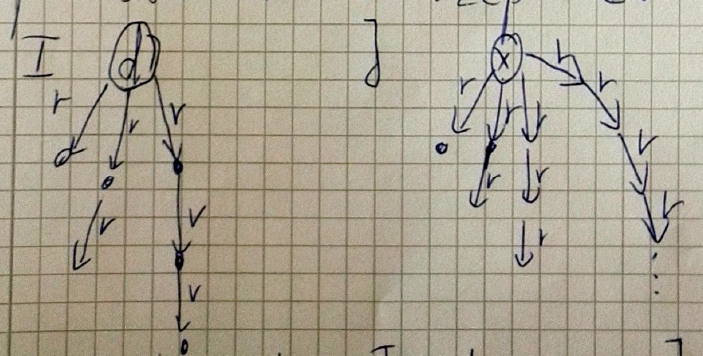
\includegraphics[width=3.71910in,height=1.83200in]{media/39bis.png}

Es gilt:

\begin{itemize}
  \item $d \in C^{\MI}$ gdw. $x \in C^{\MJ}$, falls ALC-Konzept C
  \item $(\MI,d) \not\sim (\MJ,x)$: für $y$ in $\MJ$ gibt es kein adäquates Element $e \in \Delta^{\MI}$ mit $e\ \rho\ y$
\end{itemize}

Sie gilt allerdings für verschiedene Klassen von Interpretationen, wie die Klasse aller endlichen Interpretationen oder die Klasse aller Interpretationen mit endlicher Verweigungszahl.

\subsubsection{Bisimulation für Erweiterungen von \texorpdfstring{$\ALCI$}{ALCI}}\label{bisimulation-in-alci}

Für $\ALCI$, $\ALCQ$ und $\ALCQI$ gibt es ebenfalls Bisimulationsbegriffe.

Fpr $\ALCI$ füge 2 Regeln hinzu, sodass Vorgänger auch simuliert sein müssen.

So kann man zudem zeigen, dass $\ALCI$, $\ALCQ$ und $\ALCQI$ die Baummodelleigenschaft haben.

\subsection{Ausdrucksstärke und
Modellkonstruktion}\label{ausdrucksstuxe4rke-und-modellkonstruktion}

In diesem Kapitel wird die endliche Modelleigenschaft und Filtration eingeführt.

\subsubsection{Größe von Konzepten und
TBoxen}\label{gruxf6uxdfe-von-konzepten-und-tboxen}

\begin{definition}{Größe}
\emph{Größe} $\left| C \right|$ eines ALC-Konzeptes $C$ ist induktiv
definiert:

\begin{itemize}
\item
  $\left| A \right| = 1$
\item
  $\left| \neg C \right| = \left| C \right| + 1$
\item
  $\left| C \sqcap D \right| = \left| C \sqcup D \right| = \left| C \right| + \left| D \right| + 1$
\item
  $\left| \exists r.C \right| = \left| \forall r.C \right| = \left| C \right| + 3$
\end{itemize}

\emph{Größe} $\left| C \right|$ einer TBox $\MT$ ist

\begin{itemize}
\item
  $\sum_{C \sqsubseteq D \in T}^{\left| C \right| + \left| D \right| + 1}$
\end{itemize}
\end{definition}

Intuitiv entspricht dies der Anzahl von Symbolen in $C$ bzw. $\MT$.

\subsubsection{Endliche/beschränkte Modelleigenschaft}

$\ALC$ hat \emph{endliche Modelleigenschaft}:

\begin{theorem}
Wenn ein $\ALC$-Konzept $C$ bzgl. einer $\ALC$-TBox $\MT$ erfüllbar ist, dann haben $C$ und $\MT$ ein gemeinsames \emph{endliches} Modell.
\end{theorem}

$\ALC$ hat sogar \emph{beschränkte Modelleigenschaft}:

\begin{theorem}
Wenn ein $\ALC$-Konzept $C$ bzgl. einer $\ALC$-TBox $\MT$ erfüllbar ist, dann haben $C$ und $\MT$ ein gemeinsames Modell der \emph{Kardinalität} $\leq 2^{|C|+|T|}$
\end{theorem}

\subsubsection{Typ}

Im Folgenden sei $C$ $\ALC$-Konzept und $\MT$ TBox, so dass $C$ erfüllbar bzgl. $\MT$.

Wir definieren den Begriff eines Typs:

\begin{itemize}
  \item ist Menge von Konzepten
  \item beschreibt einen Punkt $d \in \Delta^{\MI}$ in einer Interpreatation $\MI$
  \item Einschränkung auf Teilkonzepte von $C$ und $\MT$ (um Endlichkeit zu erreichen)
\end{itemize}

\subsubsection{Typ}\label{typ}

\begin{definition}{Teilkonzepte}
\begin{itemize}
\item
  $\text{sub}\left( C \right)$ ist Menge der Teilkonzepte von $C$
  (einschließlich $C$)
\item
  $\text{sub}\left( \MT \right) := \bigcup_{C \sqsubseteq D \in \MT}^{}{\text{sub}\left( C \right) \cup sub\left( D \right)}$
\item
  $\text{sub}\left( C,\MT \right) := sub\left( C \right) \cup sub\left( \MT \right)$
\end{itemize}
\end{definition}

\textbf{T3.10}

Beispiele: $$sub(\forall r.\exists r.(A \sqcap B)) = \{A,B,A \sqcap B, \exists r.(A \sqcap B), \forall r.\exists r.(A \sqcap B)\}$$
$$sub(\{A \sqsubseteq r.B, \forall r.B \sqsubseteq A\}) = \{A,B, \exists r.B, \forall r.B\}$$

\begin{lemma}

$\left| \text{sub}\left( C,T \right) \right| \leq \left| C \right| + \left| T \right|$
\end{lemma}

\begin{definition}{Typ von $d$}

Sei $\MI$ eine Interpretation, $d \in \Delta^{\MI}$. Der \emph{Typ}
$t_{\MI}\left( d \right)$ \emph{von} $d$ \emph{in} $\MI$ ist
$$t_{\MI}\left( d \right) = \left\{ D \in sub\left( C,T \right)\  \right|\ d \in D^{\MI}\}$$.
\end{definition}
Erklärung: Alle Teilkonzepte von $\MT$ und $C$, die ein Objekt $d$
erfüllt.

\textbf{T3.11}

Beispiel:

Sei $$\MT=\{A \subseteq \exists r.A\}$$
$$C = A \sqcap B$$
$$sub(C,\MT)=\{A, \exists r.A, B, A \sqcap B\}$$

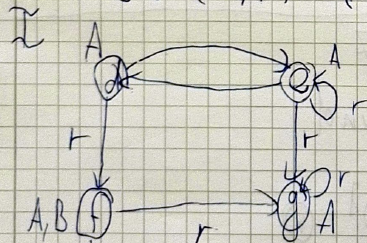
\includegraphics[width=4.71910in,height=1.83200in]{media/314typ.png}

$$t_{\MI}(d)=\{A, \exists r.A\}$$
$$t_{\MI}(e)=\{A, \exists r.A\}$$
$$t_{\MI}(f)=\{A, \exists r.A, A \sqcap B, B\}$$
$$t_{\MI}(g)=\{A, \exists r.A\}$$ \\

\begin{lemma}

Für jede Interpretation $\MI$ gilt:
$\#\left\{ t_{\MI}\left( d \right)\ |\ d \in \Delta^{\MI} \right\} \leq 2^{\left| C \right| + |T|}$
\end{lemma}

\subsubsection{Filtration}\label{filtration}

Idee:

\begin{itemize}
  \item Gegeben Interpretation $\MI$, indentifiziere alle Elemente gleichen Typs
  \item Danach kommt also jeder Typ nur einmal vor
  \item Nach Lemma 3.15 gibt es nur $2^{|C|+|\MT|}$ viele Typen
  \item Wenn $\MI$ Modell von $C$ und $\MT$, so auch das Resultat.
\end{itemize}

\begin{definition}{Filtration}

Sei $\MI$ Interpretation. Definiere Äquivalenzrelation $\sim$ auf
$\Delta^{\MI}$: $$d \sim e\ gdw.\ t_{\MI}\left( d \right) = t_{\MI}\left( e \right)$$
Wir bezeichnen diese Äquivalenzklasse von $d \in \Delta^{\MI}$ bzgl. $\sim$ mit $\left\lbrack d \right\rbrack$.

Die Filtration von $\MI$ bzgl. $C$ und $\MT$ ist folgende Interpretation $\MJ$:

\begin{itemize}
\item
  $\Delta^{\MJ} = \left\{ \left\lbrack d \right\rbrack\ |\ d \in \Delta^{\MI} \right\}$
\item
  $A^{\MJ} = \left\{ \left\lbrack d \right\rbrack\ |\ d \in A^{\MI} \right\}$
  für alle $A \in sub\left( C,\MT \right)$
\item
  $r^{\MJ} = \left\{ \left( \left\lbrack d \right\rbrack,\left\lbrack e \right\rbrack \right)|\ \exists d^{'} \in \left\lbrack d \right\rbrack,\ e^{'} \in \left\lbrack e \right\rbrack:\left( d^{'},e^{'} \right) \in r^{\MI} \right\}$
  für alle Rollennamen $r$
\end{itemize}

Beachte: $A^{\MJ}$ ist wohldefiniert (Repräsentantenunabhängigkeit)
\end{definition}

\textbf{T3.11cont}

Wenden wir diese Definition auf das Beispiel T3.11 an.

$$[d]=\{d,e,g\}$$
$$[f]=\{f\}$$

Die Interpretation $\MJ$ sieht wie folgt aus:

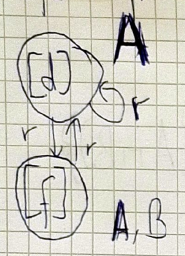
\includegraphics[width=1.21910in,height=2.33200in]{media/314typcont.png}

Offensichtlich bringt Filtration aber nicht immer das minimalste Modell, denn folgende Interpretation wäre auch ein Modell:

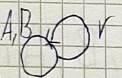
\includegraphics[width=1.0in,height=1.0in]{media/314typcont2.png}

\begin{theorem} 
Wenn $\MI$ Modell von $C$ und $\MT$, so auch $\MJ$, bzw. für alle
$d \in \Delta^{\MI}$ und $D \in sub(C,\MT)$ gilt: $d \in D^{\MI}$ gdw.
$\left\lbrack d \right\rbrack \in D^{\MJ}$.
\end{theorem}

\textbf{T3.12}

\begin{proof}
Beh.: Für alle $d \in \Delta^{\MI}$ und $D \in sub(C,\MT)$ gilt: $$d \in D^{\MI}\ gdw.\ \left\lbrack d \right\rbrack \in D^{\MJ}*$$

Beweis per Induktion über die Struktur von $D$.

\textbf{I.A.} $C = A$ * folgt aus Definition $A^{\MJ}$.

\textbf{I.S.}

\begin{enumerate}
\def\labelenumi{\arabic{enumi}.}
\item
  $\neg$, $\sqcap$ einfach mittels Semantik und I.A.
\item
  $D = \exists r.E$

  \begin{enumerate}
  \def\labelenumii{\alph{enumii}.}
  \item
    Hinrichtung

\begin{quote}
$d \in \left( \exists r.E \right)^{\MI}$ \\
$\Leftrightarrow$ (Semantik) es gibt $e \in \Delta^{\MI}$ mit $\left( d,e \right) \in r^{\MI}$ und $e \in E^{\MI}$ \\
$\Rightarrow$ (Definition $r^{\MJ}$ und I.V.) es gibt $e \in \Delta^{\MI}$ mit $\left( \left\lbrack d \right\rbrack,\left\lbrack e \right\rbrack \right) \in r^{\MJ}$ und $\left\lbrack e \right\rbrack \in E^{\MJ}$ \\
$\Leftrightarrow$ (Semantik $\exists$) $\left\lbrack d \right\rbrack \in \left( \exists r.E \right)^{\MJ}$
\end{quote}

\def\labelenumi{\alph{enumi}.}
\item
  Rückrichtung

\begin{quote}
$\left\lbrack d \right\rbrack \in \left( \exists r.E \right)^{\MJ}$ \\
$\Leftrightarrow$ (Semantik $\exists$) es gibt $[e] \in \Delta^{\MJ}$ mit $\left( \left\lbrack d \right\rbrack,\left\lbrack e \right\rbrack \right) \in r^{\MJ}$ und $\left\lbrack e \right\rbrack \in E^{\MJ}$ \\
$\Leftrightarrow$ (Definition $r^{\MJ}$ und I.V.) es gibt $[e] \in \Delta^{\MJ}$, es gibt $d^{'} \in \left\lbrack d \right\rbrack$, $e^{'} \in \left\lbrack e \right\rbrack$, $\left( d^{'},\ e^{'} \right) \in r^{\MI}$ und $e^{'} \in E^{\MI}$ \\
$\Rightarrow$ (Semantik $\exists$) $d^{'} \in \left( \exists r.E \right)^{\MI}$ \\
$\Rightarrow$ ($d \sim d^{'}$) $d \in \left( \exists r.E \right)^{\MI}$
\end{quote}

\end{enumerate}
\end{enumerate}
\end{proof}

Sei $d \in C^{\MI}$. Nach Behauptung gilt $[d] \in C^{\MJ}$, also ist $\MJ$ Modell von $C$.

$\MJ$ ist ebenfalls Modell von $\MT$:

Sei $C \sqsubseteq D$ in $\;T$, $[d] \in C^{\MJ}$ \\
Nach Beh. gilt $d \in C^{\MI}$ \\
Weil $\MI$ Modell von $C \sqsubseteq D$, gilt $d \in D^{\MI}$ \\
Nach Beh. gilt $[d] \in D^{\MJ}$

\subsubsection{Endliche/Beschränkte Modelleigenschaft}

\textbf{Theorem 3.11} \\
Wenn ein $\ALC$-Konzept $C$ bzgl. einer $\text{$\ALC$-TBox}$ $\MT$ erfüllbar ist, dann haben $C$ und $\MT$ ein gemeinsames Modell der
\emph{Kardinalität} $\leq 2^{\left| C \right| + |\MT|}$.

Beweis. Folgt aus Theorem 3.17 und Lemma 3.15.

Ähnliches (mit der selben Schranke) lässt sich für $\ALCI$ und $\ALCQ$ beweisen. (mit derselben Schranke)

\begin{theorem}
$\ALCQI$ hat nicht die endliche Modelleigenschaft.
\end{theorem}

Beweis: $A$ hat nur unendliche Modelle bzgl. folgender TBox:

\begin{itemize}
\item
  $\top \sqsubseteq \exists r.\neg A$
\item
  $T \sqsubseteq ( \leq 1\ r^{-}\ \top)$
\end{itemize}

\textbf{T3.13}

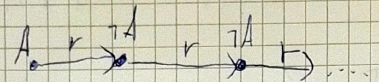
\includegraphics[width=3.21910in,height=0.93200in]{media/318qi.png}

Erklärung: Diese Interpretation müsste unendlich erweitert werden, damit es die TBox erfüllt.

\subsubsection{Entscheidbarkeit}
\textbf{Theorem 3.11}:

Wenn $C$ erfüllbar bzgl. $\MT$, dann haben $C$ und $\MT$ Modell der
Größe $\leq 2^{\left| C \right| + \left| T \right|}$.

Erfüllbarkeit ist also entscheidbar:

Gegeben $C$ und $\MT$, so dass $|C|+|\MT| = n$,
\begin{itemize} 
  \item erzeuge alle Interpretationen $\MI$ mit $\left| \Delta \right|^{\MI} \leq 2^{n}$ (es gibt höchstens $2^{2^{5n}}$ viele davon) 
  \item und überprüfe, ob $\MI$ Modell von $C$ und $\MT$ ist. (in Zeit polynomiell in $\MI$, $C$, und $\MT$)
\end{itemize}

\begin{lemma}
Gegeben sei ein $\ALC$-Konzept $C$ und endliche Interpretation $\MI$. Man kann in polynomieller Zeit -- genauer in Zeit $O\left( \left| C \right| \cdot \left| \Delta^{\MI} \right| \right)$ -- die Extension $C^{\MI}$ berechnen.
\end{lemma}

Beweisskizze zu Lemma 3.19: Rekursiver Algorithmus über die Definition der Konzeptsemantik. Dessen Zeitaufwand ist $\mathcal{O}(|C| \cdot |\Delta^{\MI}|)$:

\begin{itemize}
  \item Anzahl der (rekursiven Aufruf $= |sub(C)| \leq |C|$)
  \item pro Aufruf Zeitaufwand $\mathcal{O}(|\Delta^{\MI}|)$: \\
  simple Operationen auf $\leq 2$ Teilmengen von $\Delta^{\MI}$
\end{itemize}

\begin{korollar}
Gegeben seien $C$, $\MT$ in $\ALC$ und endliche Interpretation $\MI$. Man kann in polynomieller Zeit -- genauer: in Zeit $O(\left( \left| \MT \right| + \left| C \right| \right) \cdot \left| \Delta^{\MI} \right|)$ -- entscheiden, ob $\MI$ ein Modell von $C$ und $\MT$ ist.
\end{korollar}

\begin{theorem}
In $\ALC$ ist Erfüllbarkeit bzgl. TBoxen entscheidbar.
\end{theorem}

Die Komplexität liegt aber bei 2-ExpTime: 2-exponentiell viele Interpreationen müssen geprüft werden, jede Prüfung braucht polynomielle Zeit.

Dieser Ansatz ist kaum tauglich für die Praxis.

	\newpage

	\section{Tableau-Algorithmen}
	\subsection{Ziel}

Automatisches Schlussfolgern spielt eine zentrale Rolle für BLen. Insbesondere ist die Ausdruckstärke von BLen stark darauf zugeschnitten.

Dabei ist aber wichtig, dass die relevanten Schlussfolgerungsprobleme entscheidbar sind, sie ein möglichst geringe Komplexität haben und/oder Algorithmen existieren, die sich in der Praxis performant verhalten.

Von uns wird hauptsächlich das Problem der Erfüllbarkeit betrachtet.

In der Praxis haben sich hauptsächlich Tableau-Algorithmen und Resolutionsverfahren als effizient herausgestellt.

\subsection{ALC ohne TBoxen}\label{alc-ohne-tboxen}

\subsubsection{Negationsnormalform}\label{negationsnormalform}

\begin{definition}{Negationsnormalform}

Konzept ist in \emph{Negationsnormalform} (NNF) gdw. Negation nur auf
Konzeptnamen angewendet wird.
\end{definition}

\begin{lemma}
Jedes Konzept kann in Linearzeit in ein äquivalentes Konzept in NNF
umgewandelt werden.
\end{lemma}

\textbf{T4.1}

Beweisskizze. Wende Gesetze der doppelten Negation, de Morgan und
Dualität von $\exists$, $\forall$ an.

\subsubsection{I-Baum}\label{i-baum}

\begin{definition}{I-Baum}

\emph{I-Baum} für $C_{0}$ (in NNF) ist knoten- und kantenbeschrifteter
Baum $\left( V,E,L \right)$ mit

\begin{itemize}
\item
  $V$ Knotenmenge
\item
  $E$ ist Menge beschrifteter Kanten $\left( v,r,v^{'} \right)$ mit
  $v$,$\ v^{'} \in V$, $r$ Rollenname
\item
  $L$: $V \rightarrow 2^{sub(C_{0})}$
\end{itemize}
\end{definition}

\textbf{T4.2}

Bsp. $$C_0 = A \sqcap \forall r.(\neg A \sqcap \exists r.B)$$
$$sub(C_0) = \{A, \neg A, B, \exists r.B, \neg A \sqcap \exists r.B, \forall r.(\neg A \sqcap \exists r.B)\}$$

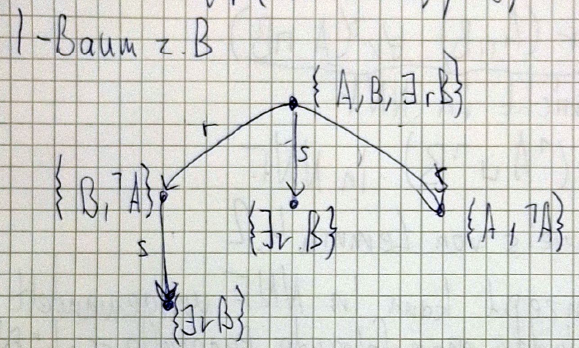
\includegraphics[width=3.71910in,height=1.83200in]{media/42ibaum.png}

\subsubsection{Tableau-Algorithmus}\label{tableau-algorithmus}

Berechnet Folge $$M_{0},M_{1},\ldots$$ von Mengen von I-Bäumen:

$$M_{0} = \left\{ B_{\text{ini}} \right\}\ mit\ B_{\text{ini}}\ \emph{initialer I-Baum}\ fuer\ C_{0}:$$

\begin{itemize}
\item
  $V := \left\{ v_{\text{ini}} \right\}$
\item
  $E := \emptyset$
\item
  $L := \left( v_{\text{ini}} \right) \left\{ C_{0} \right\}$
\end{itemize}

$M_{i + 1}$ entsteht aus $M_{\MI}$ durch Anwendung der Tableau-Regeln
auf irgendeinen I-Baum in $M_{\MI}$ und anschließendes Austauschen des
verwendeten Baumes durch den neu erzeugten (Sei $\left( V,E,L \right)$
I-Baum):

\begin{itemize}
\item
  $\sqcap$-Regel

  \begin{itemize}
  \item
    Wähle $v \in V$ und $C \sqcap D \in L\left( v \right)$ so dass
    \emph{nicht} $\left\{ C,D \right\}\  \subseteq L\left( v \right)$
  \item
    erweitere $L(v)$ um $C$ und $D$
  \end{itemize}
\item
  $\sqcup$-Regel

  \begin{itemize}
  \item
    Wähle $v \in V$ und $C \sqcup D \in L\left( v \right)$ so dass
    $\left\{ C,D \right\}\  \cap L\left( v \right) = \varnothing$
  \item
    erweitere $L(v)$ um $C$ oder $D$ (ergibt zwei I-Bäume)
  \end{itemize}
\item
  $\exists$-Regel

  \begin{itemize}
  \item
    Wähle $v \in V$ und $\exists r.C \in L\left( v \right)$ so dass
    es kein $v^{'} \in V$ gibt mit $\left( v,r,v^{'} \right) \in E$
    und $C\  \in L\left( v' \right)$
  \item
    erweitere V um neuen Konten $v^{'}$ und $E$ um
    $\left( v,r,v^{'} \right)$; setze
    $L\left( v^{'} \right) = \left\{ C \right\}$
  \end{itemize}
\item
  $\forall$-Regel

  \begin{itemize}
  \item
    Wähle $v,v^{'} \in V$ und $\forall r.C \in L\left( v \right)$ so
    dass $\left( v,r,v^{'} \right) \in E$ und
    $C\  \notin L\left( v \right)$
  \item
    erweitere $L(v')$ um $C$
  \end{itemize}
\end{itemize}

Stoppe, wenn alle Regeln erschöpfend angewandt wurden. Gib „erfüllbar``
zurück, falls es einen I-Baum ohne offensichtlichen Widerspruch
($\left\{ A,\neg A \right\} \subseteq L\left( v \right)$) gibt;
„unerfüllbar`` sonst.

\textbf{T4.3}

Beispiel:

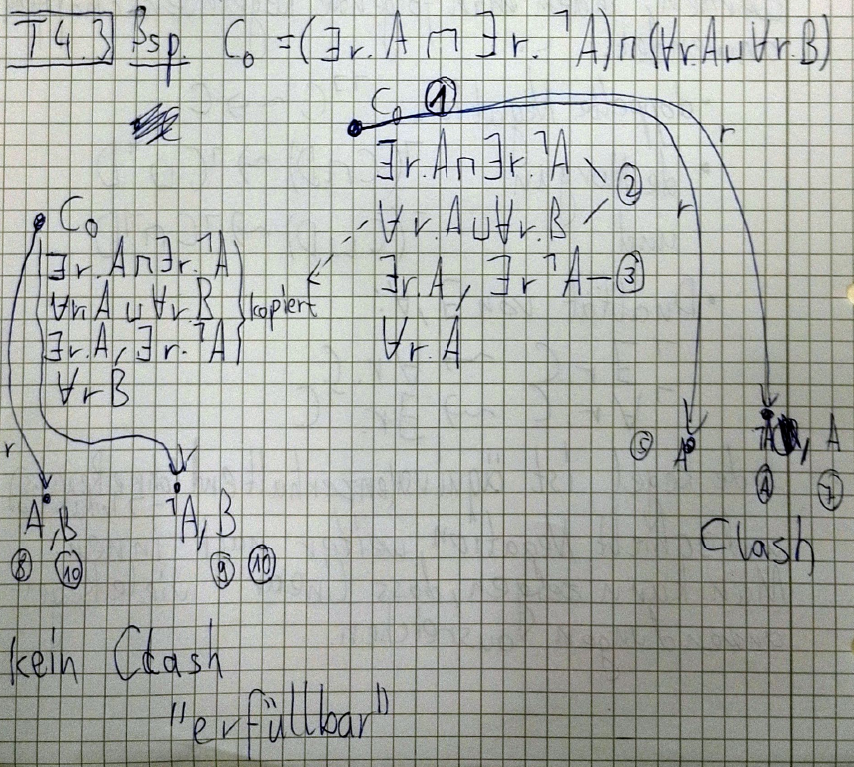
\includegraphics[width=5.71910in,height=3.83200in]{media/43taleau.png}

\subsubsection{Definition Rollentiefe}\label{definition-rollentiefe}

Rollentiefe $\text{rd}\left( C \right)$ von Konzepten
$C \in sub\left( C_{0} \right)$ ist induktiv definiert:

\begin{itemize}
\item
  $\text{rd}\left( A \right) = rd\left( \neg A \right) = 0$
\item
  $\text{rd}\left( C \sqcap D \right) = rd\left( C \sqcup D \right) = \max\left( \text{rd}\left( C \right),rd\left( D \right) \right)$
\item
  $\text{rd}\left( \exists r.C \right) = rd\left( \forall r.C \right) = 1 + rd\left( C \right)$
\end{itemize}

\begin{lemma}
Für alle $C \in sub\left( C_{0} \right)$ gilt
$\text{rd}\left( C \right) \leq \left| C \right|$.
\end{lemma}

\subsubsection{Multimengen}\label{multimengen}

Multimengen sind Mengen, in denen Elemente mehrfach vorkommen dürfen, z.B.:
$$\{1,1,2,3,4,4,5,6,6,6\}$$

Formal: Multimengen über die Menge $S$ ist Abbildung $$M:S\mathbb{\rightarrow N}$$, welche jedes Element auf die Anzahl seines Vorkommens abbildet.

Die meisten Begriffe übertragen sich von Mengen auf Multimengen:

\begin{itemize}
	\item Leere Menge $\emptyset: s \mapsto 0$ für alle $s \in S$
	\item Vereinigung $(M_1 \cup M_2)(s) := M_1(s) + M_2(s)$ 
	\item Element: $s \in M\ gdw.\ M(s)>0$
	\item Differenz: $(M_1 \setminus M_2)(s) = X(m,n) = \left\{\begin{array}{lr}
        M_1(s) - M_2(s) &, wenn M_1(s) \geq M_2(s) \\
        0 & sonst
        \end{array}\right\}$
\end{itemize}

$MM(S)$ ist die Menge aller Multimengen über der Menge S.

Gegeben strikte partielle Ordnung $\left( S, < \right)$, ist die
\emph{Multimengenerweiterung} $\left( \text{MM}\left( S \right), <_{\text{mul}} \right)$ definiert als: 

$M_{2} <_{\text{mul}}M_{1}$ gdw. $\exists X,Y \in MM(S)$, so dass

\begin{itemize}
\item
  $\varnothing \neq X \subseteq M_{1}$
\item
  $M_{2} = \left( M_{1} \smallsetminus X \right) \cup Y$
\item
  $\forall y \in Y\exists x \in X : x > y$
\end{itemize}

Also erhält man $M_2$ aus $M_1$, indem man einige Elemente entfernt und durch endlich viele \emph{kleinere} ersetzt.

Beispiel:

$\left\{ 3,1 \right\} >_{\text{mul}}\{ 2,2,2\} >_{\text{mul}}\{ 2,2\} >_{\text{mul}}\{ 2,1,1,1\}$

Es ist leicht zu zeigen das diese Ordnung eine strikte partielle Ordnung ist.  Zudem ist sie wohlfundiert, wenn $(S,<)$ wohldefiniert ist: Es gibt keine unendlich $<$ absteigenden Ketten.

\setcounter{definition}{5}
\begin{theorem}

Wenn $\left( S, < \right)$ wohlfundiert (hat keine unendlichen
absteigenden Ketten) ist, dann ist auch $\left( \text{MM}\left( S \right), <_{\text{mul}} \right)$
wohlfundiert.
\end{theorem}

\setcounter{definition}{4}

\subsubsection{Terminierung}

\begin{proposition}

Der Tableau-Algorithmus stoppt nach endlicher Zeit.
\end{proposition}
\setcounter{definition}{6}

Beweis in 4 Schritten:

\begin{enumerate}
\def\labelenumi{\arabic{enumi}.}
\item
  Es werden nur I-Bäume mit einem Verzweigungsgrad
  $\leq \left| C_{0} \right|$ generiert.

\begin{quote}
\textbf{T4.5a}

Beweisskizze. Nur die $\exists$-Regel generiert Nachfolger, aber
höchstens einen für jedes Konzept $\exists r.C \in sub(C_{0})$. Nach
\protect\hyperlink{lemma-3.13}{Lemma 3.13} enthält
$\text{sub}\left( C_{o} \right)$ höchstens $\left| C_{0} \right|$
viele Konzepte.
\end{quote}

\def\labelenumi{\arabic{enumi}.}
\item
  Es werden nur I-Bäume mit einer Tiefe $\leq \left| C_{0} \right|$
  generiert.

\begin{quote}
\textbf{T4.5b}
\begin{proof}

Induktion über die Anzahl der Regelanwendungen. Zu zeigen: Wenn $v$
Knoten mit Tiefe $\MI$ ist, dann gilt
$\text{rd}\left( C \right) \leq rd\left( C_{0} \right) - i$ für alle
$C \in L\left( v \right)$.

\textbf{I.A.} Es gibt nur Knoten $v_{\text{ini}}$ mit
$L\left( v_{\text{ini}} \right) = \left\{ C_{0} \right\}$. I.V. gilt,
da $i = 0$.

\textbf{I.S.} Fallunterscheidung nach angewandter Regel (exemplarisch
$\sqcap$, $\exists$):

\begin{enumerate}
\def\labelenumi{\alph{enumi}.}
\item
  $\sqcap$-Regel

$C \sqcap D \in L(v)$ und $L(v)$ wird durch $C$, $D$ erweitert.
Nach I.V. gilt:
$\text{rd}\left( C \sqcap D \right) \leq rd\left( C_{0} \right) - i$,
also auch $\text{rd}\left( C \right) \leq rd\left( C_{0} \right) - i$,
weil $\text{rd}\left( C \right) \leq rd\left( C \sqcap D \right)$.
Analog für $D$.

\def\labelenumi{\alph{enumi}.}
\item
  $\exists$-Regel

Dann $\exists r.C \in L\left( v \right)$ und es wird neues $v^{'}$
auf Tiefe $i + 1$ generiert mit
$L\left( v^{'} \right) = \left\{ C \right\}$. Es gilt
$\text{rd}\left( C \right) = rd\left( \exists r.C \right) - 1 \leq rd\left( C_{0} \right) - i - 1 = rd\left( C_{0} \right) - (i + 1)$
 \end{enumerate}
\end{proof}
\end{quote}

\item
  Sei $M_{0},M_{1},\ldots$ die erzeugte Folge und $B \in M_{\MI}$ für
  ein $i \geq 0$. Dann ist $B$ durch die Anwendung von maximal
  $\left| C_{0} \right|^{\left| C_{0} \right|} \cdot \left| C_{0} \right| \leq 2^{2\left| C_{0} \right|^{2}} = n$ Regeln entstanden (Knoten im Baum mal Größe Knotenbeschriftung).

\end{enumerate}

Nun kann die Terminierung mittel Behauptung 3 beweisen:

\textbf{T4.5d}

\begin{proof}
Wir ordnen jedem $M_i$ eine Multimenge $MM_i$ zu. Für jedes $B \in M_i$ enthält $MM_i$ die Zahl der ``n$-$Anzahl der Regelanwendungen, mittels derer $B$ generiert wurde.''

Weil $<$ auf $\mathcal{N}$ wohldefiniert ist, ist $<_{mul}$ auf $MM(\{0,\ldots,n\})$ wohldefiniert.

Offenbar gilt $MM_{i+1} <_{mul} MM_i$ für alle $i \geq 0$ *. Also werden nur endlich oft Regeln angewendet.
\end{proof}

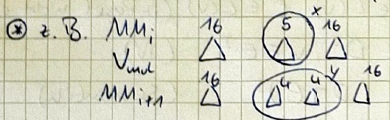
\includegraphics[width=3.71910in,height=1.83200in]{media/45mm.png}

\subsubsection{Korrektheit und Vollständigkeit}

\begin{proposition}

Wenn der Tableau-Algorithmus „erfüllbar`` zurückgibt, so ist $C_{0}$
erfüllbar.
\end{proposition}

\textbf{T4.6}

\begin{proof}

Beweis per Induktion über die Struktur von $C$.
„erfüllbar``-Ausgabe bedeutet widerspruchsfreier, vollständiger I-Baum
$B = \left( V,E,L \right)$ gefunden. Konstruiere Interpretation $\MI$:

\begin{itemize}
\item
  $\Delta^{\MI} = V$
\item
  $r^{\MI} = \left\{ \left( v,v^{'} \right) \middle| \left( v,r,v^{'} \right) \in E \right\}$
  für alle Rollennamen $r$
\item
  $A^{\MI} = \left\{ v \middle| A \in L\left( v \right) \right\}$ für
  alle Konzeptnamen $A$
\end{itemize}

Behauptung: Für alle Konzepte $C$ und $v \in V$ gilt

\begin{center}$C \in L\left( v \right)$ impliziert $v \in C^{\MI}$\end{center}

Da $C_{0} \in L\left( v_{\text{ini}} \right)$ in $B_{\text{ini}}$ gilt
auch $C_{0} \in L\left( v_{\text{ini}} \right)$ in $B$. Also
$v_{\text{ini}} \in C_{0}^{\MI}$ nach Behauptung, weswegen dann
$C_{0}$ erfüllbar.

\textbf{I.A.} $C = A$ (Konzeptname) Gilt nach Definition von
$\MI$.

\textbf{I.S.}

\begin{itemize}
\item
  $C = \neg A$

\begin{quote}
$A$ Konzeptname. Da $B$ keinen offensichtlichen Widerspruch hat,
folgt das $A \notin L(v)$. Nach Definition von $\MI$ gilt
$v \notin A^{\MI}$. Also $v \in \left( \neg A \right)^{\MI}$.
\end{quote}

\item
  $C = D \sqcap E$

\begin{quote}
$C \in L\left( v \right)$ 

$\Rightarrow$ ($\sqcap$-Regel nicht anwendbar) $D \in L\left( v \right),\ E \in L\left( v \right)$ 

$\Rightarrow$ (I.V.) $v \in D^{\MI},\ v \in E^{\MI}$ 

$\Rightarrow$ (Semantik) $v \in \left( D \sqcap E \right)^{\MI}$
\end{quote}

\item $C = D \sqcup E$

\begin{quote}
analog.
\end{quote}

\item $C = \exists r.D$

\begin{quote}
Da die $\exists$-Regel nicht anwendbar ist, gibt es $v'\in V$ mit $(v,r,v') \in E$ und $D \in L(v')$

Nach I.V.: $v' \in D^{\MI}$; nach Konstruktion $(v,v') \in r^{\MI}$. Nach Semantik gilt dann: $v \in (\exists r.D^{\MI})$
\end{quote}

\item $C = \forall r.D$
\begin{quote}
ähnlich.
\end{quote}
\end{itemize}
\end{proof}

\begin{definition}{Realisierbarkeit}

Sei $B = \left( V,E,L \right)$ ein I-Baum. Interpretation $\MI$
\emph{realisiert} $B$ gdw. es gibt eine Funktion
$\pi\ :V \rightarrow \Delta^{\MI}$ so dass

\begin{itemize}
\item
  $\left( v,r,v^{'} \right) \in E$ impliziert
  $\left( \pi\left( v \right),\pi\left( v^{'} \right) \right) \in r^{\MI}$
\item
  $C \in L\left( v \right)$ impliziert
  $\pi\left( v \right) \in C^{\MI}$
\end{itemize}

B ist \emph{realisierbar}, wenn es Interpretation $\MI$ gibt, die $B$
realisiert. Menge $M$ von I-Bäumen ist \emph{realisierbar} gdw. ein
$B \in M$ realisierbar.
\end{definition}

Beachte: realisierbarer I-Baum enthält keinen offensichtlichen Widerspruch!

\textbf{T4.7}

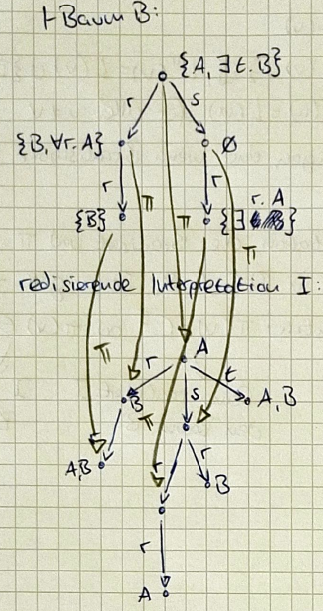
\includegraphics[width=2.0in,height=4.0in]{media/47real.png}

\begin{proposition}{Vollständigkeit}

Wenn $C_{0}$ erfüllbar, so gibt der Tableau-Algorithmus „erfüllbar``
zurück.
\end{proposition}

\textbf{T4.8}

\begin{proof}

Per Induktion über $\MI$. 

Sei $C_{0}$ erfüllbar. Nach \protect\hyperlink{proposition-4.5-terminierung}{Proposition 4.5} berechnet der Algorithmus endlich Folge $M_{0},\ldots,M_{n}$. Wir
zeigen: 

$M_{i}$ ist realisierbar für alle $0 \leq i \leq n$. 

Daraus folgt: Es gibt realisierbaren Baum $B \in M_{n}$ und damit enthält $B$ keinen offensichtlichen Widerspruch. Also gibt der Algorithmus „erfüllbar`` zurück.

\textbf{I.A.} $i = 0$. $M_{0} = {\{ B}_{\text{ini}}\}$.
$B_{\text{ini}}$ ist realisierbar, weil $C_{0}$ erfüllbar.

\textbf{I.S.} Fallunterscheidung gemäß der Regel, mit der $M_{i + 1}$
aus $M_{\MI}$ erzeugt wurde. Sei $B$ realisierbarer Baum aus
$M_i$, auf welchen Regel angewandt wird. Beispielhaft
$\sqcup$-Regel:

\begin{enumerate}
\def\labelenumi{\arabic{enumi}.}
\item
  $\sqcup$-Regel
\end{enumerate}

\begin{quote}
Dann wird $B = \left( V,E,L \right)$ ersetzt durch
$B^{'} = \left( V,E,L^{'} \right) \in M_{i + 1}$ und
$B^{''} = \left( V,E,L^{''} \right) \in M_{i + 1}$ und es gibt
$v \in V$ mit

\begin{itemize}
\item
  $\left( C \sqcup D \right) \in L(v)$
\item
  $L^{'}\left( v \right) = L\left( v \right) \cup \left\{ C \right\}$,
  $L^{''}\left( v \right) = L\left( v \right) \cup \left\{ D \right\}$
\item
  $L^{'}\left( u \right) = L^{''}\left( u \right) = L\left( u \right)$
  für alle $u \neq v$
\end{itemize}

Es genügt zu zeigen, dass wenn $B$ realisiertbar, dann $B'$ oder
$B''$ realisierbar. 

Sei $\MI$ Interpretation, die $B$ realisiert und $\pi\ :V \rightarrow \Delta^{\MI}$ Abbildung wie in \protect\hyperlink{realisierbarkeit}{Definition 4.8}. Dann gilt $\pi\left( v \right) \in \left( C \sqcup D \right)^{\MI}$. Nach Semantik: $\pi\left( v \right) \in C^{\MI}$ oder $\pi\left( v \right) \in D^{\MI}$. Also realisiert $\MI$ den Baum $B'$ oder $B''$.
\end{quote}
\end{proof}

\subsubsection{Komplexitätsanalyse}\label{praktikabilituxe4t}

Wir beobachten: 

I-Bäume können höchstens exponentiell groß werden.

Dieser Fall kann tastsächlich eintreffen. Beispielhaft, der Erfüllbarkeitstest von:
$$\bigsqcap_{i < n} \forall r^i .(\exists r.B \sqcap \exists r.\neg B)$$
generiert Baum der Größe $2^n$.

Also: exponentieller Zeit- und Platzverbrauch (sogar 2-exponentiell)

\subsubsection{Praktikabilität}

Offenbar wäre eine naive Implementierung nicht effizient. Dabei kann man aber einige Hinweise/Optimierungen bei der Implementierung beachten:

\begin{itemize}
	\item Es wird nur ein Baum zur Zeit generiert, keine Menge
	\item bei der $\sqcup$-Regel muss man sich also entscheiden (Heuristik); ggf. Entscheidung revidiieren (Backtracking).
	\item Es wird nur ein Teil des Baumes (Pfad) im Speicher gehalten.
	\item Backjumping: Führe Buch über die ``Herkunft'' von Knotenbeschriftungen und Kanten mittels Dependenzmengen. Wenn Backtracking nötig, springe direkt zu einer der Ursachen des Widerspruches zurück.
\end{itemize}

\subsection{ALC mit generellen TBoxen}\label{alc-mit-generellen-tboxen}

Nun wollen wir einen Tableau-Algorithmus für die Erfüllbarkeit in $\ALC$  \emph{bzgl. TBoxen}.

Jede TBox $\MT$ ist äquivalent zu einer TBox der Form
$\left\{ \top \sqsubseteq C_{\MT} \right\}$: 

\begin{center}setze $C_{\MT} := \prod_{C \sqsubseteq D \in \MT}^{}{\neg C \sqcup D}$.\end{center}

\textbf{T4.11} Beispiel

$$\MT = \{A \sqsubseteq \exists r.B, A \sqcup B \sqsubseteq \forall r.B\}$$

Daraus wird

$$\{\top \sqsubseteq (\neg A \sqcup \exists r.B) \sqcap (\neg (A \sqcup B) \sqcup \forall r.B)\}$$

in NNF:

$$\MT' = \{\top \sqsubseteq (\neg A \sqcup \exists r.B) \sqcap ((\neg A \sqcap \neg B) \sqcup \forall r.B)\}$$

Desweiteren nehmen wir an, dass:

\begin{itemize}
	\item Eingabe $C_0$ in NNF;
	\item Eingabe $\MT$ hat Form $\{\top \sqsubseteq C_{\MT}\}$ mit $C_{\MT}$ in NNF
\end{itemize}

Nun modifiziere den vorigen Algorithmus durch Hinzufügen folgender Regel:

\subsubsection{TBox-Regel}\label{tbox-regel}

Wähle $v \in V$ so dass $C_{\MT} \notin L\left( V \right)$ und
erweitere $L\left( v \right)$ um $C_{\MT}$.

Problem: Terminiert nicht!

\textbf{T4.12}

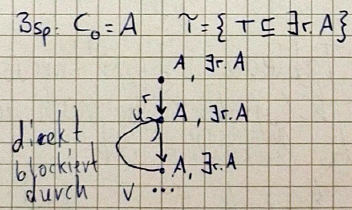
\includegraphics[width=3.71910in,height=1.83200in]{media/412endl.png}

\subsubsection{Blockieren}\label{blockieren}

Dies lösen wir, indem wir nur ein endliches Anfangsstück eines Baummodells anhand dessen sich die Existenzeines vollständigen Modells entscheiden lässt konstruieren. Dazu müssen wir die Anwendung der $\exists$-Regel einschränken.

\begin{definition}{Blockiert}

Sei $\left( V,E,L \right)$ ein I-Baum und $u,v \in V$. Dann ist
$v$ direkt blockiert durch $u$, wenn

\begin{enumerate}
\def\labelenumi{\arabic{enumi}.}
\item
  $u$ Vorgänger von $v$ in $B$ ist und
\item
  $L\left( v \right) \subseteq L\left( u \right)$
\end{enumerate}

$v$ ist blockiert, wenn $v$ direkt blockiert ist oder einen direkt
blockierten Vorgänger hat.
\end{definition}

\subsubsection{\texorpdfstring{Neue $\exists$-Regel
($\exists^{'}$-Regel)}{Neue \textbackslash{}exists-Regel (\textbackslash{}exists\^{}\{'\}-Regel)}}\label{neue-exists-regel-exists-regel}

\begin{itemize}
\item
  Wähle $v \in V$ und $\exists r.C \in L\left( v \right)$ so dass
  $v$ \emph{nicht blockiert ist und} es kein $v^{'} \in V$ gibt mit
  $\left( v,r,v^{'} \right) \in E$ und $C\  \in L\left( v' \right)$
\item
  erweitere V um neuen Konten $v^{'}$ und $E$ um
  $\left( v,r,v^{'} \right)$; setze
  $L\left( v^{'} \right) = \left\{ C \right\}$
\end{itemize}

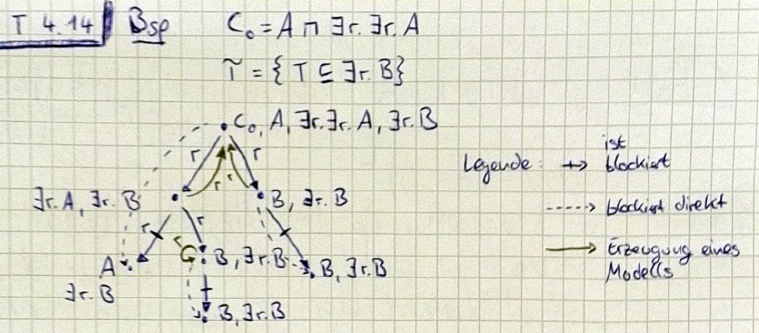
\includegraphics[width=5.71910in,height=2.33200in]{media/414block.png}

\subsubsection{Vollständigkeit}\label{vollstuxe4ndigkeit}

\begin{proposition}
Wenn $C_0$ erfüllbar bzgl. $\MT$, so gibt der Algorithmus erfüllbar zurück.
\end{proposition}

Beweis wie ohne TBoxen: Alle $M_{0},\ldots,\ M_{n}$ sind realisierbar
bzgl. $\MI$ (Induktion), also enthält $M_{n}$ einen Baum ohne
offensichtlichen Widerspruch (Nur neue Fallunterscheidung für TBox-Regel und Realisierbarkeitsbegriff auf TBoxen erweitert).

\subsubsection{Korrektheit}\label{korrektheit}

\begin{proposition}
Wenn der Algorithmus ``erfüllbar'' zurückgibt, so ist $C_0$ erfüllbar bzgl. $\MT$
\end{proposition}

\textbf{T4.15}

Beweisskizze per Induktion über die Struktur von $C$. Definiere
Interpretation $\MI$:

\begin{itemize}
\item
  $\Delta^{\MI} = \left\{ v \in V \middle| \text{v\ }\mathrm{\text{nicht\ blockiert}} \right\}$
\item
  $r^{\MI} = \left\{ \left( v,v^{'} \right)\  \middle| \ \left( v,r,v^{'} \right) \in E \right\} \cup \left\{ \left( v,u \right)\  \middle| \ \exists\left( v,r,v^{'} \right) \in E\mathrm{\ }\mathrm{\text{und}}\mathrm{\ }v^{'}\mathrm{\ }\mathrm{\text{direkt\ blockiert\ durch}}\mathrm{\ }u \right\}$
\item
  $A^{\MI} = \left\{ v \middle| A \in L\left( v \right) \right\}$
\end{itemize}

Behauptung: Für alle ALC-Konzepte $C$ und $v \in \Delta^{\MI}$ gilt:
$$C \in L\left( v \right) \Rightarrow v \in C^{\MI}$$
Die Behauptung impliziert wie gewünscht, dass

\begin{itemize}
\item
  $\MI$ Modell von $\MT$ ist.

Da die TBox-Regel nicht anwendbar ist, gilt $C_{\MT} \in L\left( v \right)$ für alle $v \in V$. Also $v \in C_{\MT}^{\MI}$ für alle $v \in \Delta^{\MI}$.

\item
  $\MI$ Modell von $C_{0}$ ist.

Da $C_{0} \in L\left( v_{\text{ini}} \right)$ gilt nach Behauptung
$v_{\text{ini}} \in C_{0}^{\MI}$.
\end{itemize}

\textbf{I.A.} Siehe Beweis zu
\protect\hyperlink{proposition-4.7-korrektheit}{Proposition 4.7}.

\textbf{I.S.} Schritte wie in Beweis zu Proposition 4.7, außer:

\begin{itemize}
\item
  $C = \exists r.D$
\end{itemize}

Sei $\exists r.D \in L\left( v \right)$. Da die $\exists'$-Regel
nicht anwendbar ist, gibt es $v^{'} \in V$ mit
$\left( v,r,v^{'} \right) \in E$ und $D \in L\left( v \right)$.
Fallunterscheidung:

\begin{enumerate}
\def\labelenumi{\arabic{enumi}.}
\item
  $v'$ unblockiert. Dann $\left( v,v^{'} \right) \in r^{\MI}$
  (Definition $\MI$), $v^{'} \in D^{\MI}$ (\textbf{I.V.})
  $\Rightarrow v \in \left( \exists r.D \right)^{\MI}$
\item
  $v^{'}$ blockiert. Da der direkte Vorgänger $v$ von $v'$
  unblockiert ist, ist $v'$ direkt blockiert von unblockiertem
  Vorgänger $u$. Es gilt:
\end{enumerate}

\begin{itemize}
\item
  $\left( v,u \right) \in r^{\MI}$ nach Definition $r^{\MI}$
\item
  $D \in L\left( v \right) \subseteq L\left( u \right)$
  (Blockierungsbedingung)
\item
  $\Rightarrow u \in D^{\MI}$ (\textbf{I.V.})
\end{itemize}

\begin{quote}
Also $v \in \left( \exists r.D \right)^{\MI}$.
\end{quote}

\begin{itemize}
\item
  $C = \forall r.D$
\end{itemize}

Ähnlich zu oberem Fall.

\subsubsection{Terminierung}\label{terminierung}

\begin{proposition}
Der Tableau-Algorithmus stoppt nach endlicher Zeit.
\end{proposition}

Beweis analog zu den ohne TBoxen (Prop. 4.5), aber mit Einbezug der TBox. Wir zeigen es also in den selben Schritten:

Beweis in 4 Schritten:

\begin{enumerate}
\def\labelenumi{\arabic{enumi}.}
\item
  Es werden nur I-Bäume mit einem Verzweigungsgrad $\leq \left| C_{0} \right| + \color{red} \left| \MT \right|$ generiert.
\item
  Es werden nur I-Bäume mit einer Tiefe $\color{red} 2^k$ generiert.
  \begin{quote}
  \textbf{T4.16}

  Angenommen, es wird ein I-Baum der Tiefe $> 2^k$ erzeugt.

  Dann wird irgendwann die $\exists '$-Regel auf einen Knoten $v$ der Tiefe $2^k$ angewendet.

  Betrachte Pfad $v_0, \ldots , v_{2^k}$ von der Wurzel bis v. Dieser Pfad hat $2^k+1$ Knoten.

  Weil es nur $2^k$ möglich Knotenbeschriftungen gibt, muss es auf dem Pfad zwei Knoten $v_i$ und $v_j$ geben, mit $0 \leq i < j \leq 2^k$, welche dieselben Knotenbeschriftungen haben, also $L(v_i) = L(v_j)$. Also ist $v_j$ durch $v_i$ blockiert, weswegen auch $v$ blockiert ist. $\lightning$

  Widerspruch zur Anwendung der $\exists '$-Regel auf $v_j$, also ist die Annahme falsch.
  \end{quote}
\item
  Sei $M_{0},M_{1},\ldots$ die erzeugte Folge und $B \in M_{\MI}$ für
  ein $i \geq 0$. Dann ist $B$ durch die Anwendung von maximal
  $\color{red} k^{2^{k}} \cdot k \leq 2^{2^{3k}}= n$ Regeln entstanden (Knoten im Baum mal Größe Knotenbeschriftung).
\end{enumerate}

Danach kann Terminierung wie gehabt mittels Behauptung 3 bewiesen werden.

\subsubsection{Komplexität}

Im Beweis zum 3. Schritt der Terminierung haben wir gesehen, dass die I-Bäume höchstens doppelt exponentiell groß werden.

Dieser Worst-Case kann eintreten!

\begin{lemma}
Es gibt Eingabe $C_0$, $\MT$ für die der Tableau-Algorithmus einen Baum von exponentieller Tiefe generiert.
\end{lemma}

Also: 2-exponentieller Zeit- und Platzaufwand (sogar 3-exponentiell!).

\subsubsection{Bemerkung zur TBox-Regel}

TBoxen führen zu Backtracking:

\begin{center}Normalisierung von $\MT$ zu $\{\top \sqsubseteq \bigsqcap_{C \sqsubseteq D \in \MT} \neg C \sqcup D\}$\end{center}

Daher wird jede $\sqcup$-Regel für \emph{Konzeptinklusion} auf \emph{jeden} Knoten angewendet!

Also braucht man für eine effiziente Implementierung Optimerungstechniken, die die Dijsunktionen, soweit möglich, eliminieren (``Absorption'').

\subsubsection{Erweiterungen}

Der Algorithmus kann auch auf $\ALCI$, $\ALCQ$ und $\ALCQI$ erweitert werden.

Das ist teilweise subtiler als erwartet, z.B.:

\begin{itemize}
	\item $\ALCI$
	Offensichtlich: Hinzufügen von Regeln für $\exists r^{-}.C$ und $\forall r^-.C$

	Weniger offensichtlich Blockierungsbedingungen muss verschärft werden, sonst ist Algorithmus nicht korrekt.
\end{itemize}

Für $\ALCQI$ ist eine noch aufwendigere Blockierungsbedingung nötig.
	\newpage

	\section{Komplexität}
	\subsection{Komplexität mit TBoxen, obere
Schranke}\label{komplexituxe4t-mit-tboxen-obere-schranke}

\subsubsection{Obere Schranke}

Wir wollen zeigen:

\begin{theorem}
In $\ALC$ ist die Erfüllbarkeit von Konzepten bzgl. TBoxen
ExpTime-Vollständig.
\end{theorem}

Mit Lemma 2.9: Subsumtion und Äquivalenz ExpTime-Vollständig.

Wir beginnen mit oberer Schranke (Enthaltensein in ExpTime):

\begin{itemize}
  \item wir verwenden ein Verfahren aus der Modallogik: Typelimination
  \item basiert auf syntaktischem Typ-Begriff
\end{itemize}

\subsubsection{Syntaktische Typen}\label{synt-typ}

Wir nehmen an, dass das Eingabe-Konzept $C_0$ in NNF ist und die Eingabe-TBox die Form $\{\top \sqsubseteq C_{\MT}\}$ hat mit $C_{\MT}$ in NNF.

\begin{definition}{Typ}

Ein Typ für $C_{0}$ und $T$ ist Teilmenge
$t \subseteq sub\left( C_{0},T \right)$, so dass

\begin{enumerate}
\def\labelenumi{\arabic{enumi}.}
\item
  $A \in t$ gdw. $\neg A \notin t$ für alle
  $\neg A \notin sub\left( C_{0},T \right)$
\item
  $C \sqcap D \in t$ gdw. $C \in t$ und $D \in t$ für alle
  $C \sqcap D \in sub\left( C_{0},T \right)$
\item
  $C \sqcup D \in t$ gdw. $C \in t$ oder $D \in t$ für alle
  $C \sqcup D \in sub\left( C_{0},T \right)$
\item
  $C_{T} \in t$
\end{enumerate}
\end{definition}

\textbf{T5.1}

Beispiel:

$C_0 = A$, $\MT = \{\top \subseteq C_{\MT}\}$ mit $$C_{\MT} = \exists r.\exists r.A \sqcap \forall r.A' \sqcap (\neg A \sqcup \neg A')$$

Dann ist $$sub(C_0, \MT) = \{A, C_{\MT}, \exists r.\exists r.A, \forall r.A',\neg A \sqcup \neg A', \exists r.A, A', \neg A, \neg A'\}$$

Sei $M = \{C_{\MT}, \exists r.\exists r. A, \forall r.A', \neg A \sqcup \neg A'\}$

Die Typen für $C_0$ und $\MT$ sind:

\begin{itemize}
  \item $t_0 = M \cup \{\neg A, \neg A'\}$
  \item $t_1 = M \cup \{\neg A, A'\}$
  \item $t_2 = M \cup \{A, \neg A'\}$
  \item $t_0' = M \cup \{\exists r.A\}$
  \item $t_1' = M \cup \{\exists r.A\}$
  \item $t_2' = M \cup \{\exists r.A\}$
\end{itemize}

\subsubsection{Typelimination}\label{typelimination}

Die generelle Idee der Typelimination bei Eingabe $C_0$, $\MT$:

\begin{enumerate}
\def\labelenumi{\arabic{enumi}.}
\item
  Generiere alle Typen für $C_{0}$ und $T$ (exponentiell viele)
\item
  Eliminiere wiederholt Typen, die in keinem Modell von $T$ vorkommen
  können
\item
  Überprüfe, ob ein Typ überlebt hat, der $C_{0}$ enthält
\item
  Wenn ja, antworte „erfüllbar``, sonst „unerfüllbar``
\end{enumerate}

\subsubsection{Schlechte Typen}\label{schlechter-typ}

Wir formalisieren ``Typen, die in keinem Modell vorkommen können''.

\begin{definition}{schlechter Typ}

Sei $\Gamma$ Typenmenge und $t \in \Gamma$.

Dann ist $t$ \emph{schlecht in} $\Gamma$, wenn für ein $\exists r.C \in t$ gilt:

\begin{center}Es gibt kein $t^{'} \in \Gamma$ mit
$\left\{ C \right\} \cup \left\{ \text{D\ } \middle| \ \forall r.D \in t \right\} \subseteq t^{'}$.\end{center}
\end{definition}

Erklärung: $t$ braucht einen ``Zeugen'', es gibt aber keinen
geeigneten.

\textbf{T5.1cont}

Beispielsweise ist $t_0'$ schlecht in der Menge $\{t_0,t_1,t_2,t_0',t_1',t_2'\}$. Für $\exists r.A \in t_0'$ ist die Menge aus Definition 5.3 $\{A,A'\}$. Kein Typ enhält $A$ und $A'$. Analog: $t_1'$, $t_2'$ sind schlecht. Entfernt man diese drei so erhält man die Menge $\Gamma_1 = \{t_1,t_2,t_2\}$. 

Nun sind aber $\{t_1,t_2,t_3\}$ schlecht in $\Gamma_1$: Sie enthalten $\exists r. \exists r.A$ , aber kein Typ in $\Gamma_1$ enthält $\exists r.A$.

\begin{proposition}
$\ALC$-Elim($C_0,\MT$) terminiert nach $2^{\mathcal{O}(|C_0|+|\MT|)}$ Schritten.
\end{proposition}

\textbf{T5.2}

\begin{proof}
Sei $n = \left| C_{0} \right| + |T|$. Proposition folgt aus:

\begin{enumerate}
\def\labelenumi{\arabic{enumi}.}
\item
  Es gibt nur $2^{n}$ Typen mit $n \left| C_{0} \right| + T$
  (\protect\hyperlink{lemma-3.15}{Lemma 3.15})
\item
  In jedem Schritt, der repeat-Schleife wird mindestens ein Typ
  eliminiert; die Schleife terminiert spätestens nach $2^{n}$
  Durchläufen.
\item
  Die restlichen Operationen (prüfen, ob ein Typ schlecht ist usw.)
  können leicht in Zeit $2^{O\left( n \right)}$ implementiert werden.
\end{enumerate}
\end{proof}

\begin{proposition}
$\ALC$-Elim($C_0,\MT$) antwortet ``erfüllbar'' gdw. $C_0$ erfüllbar bzgl. $\MT$
\end{proposition}

\textbf{T5.3}. 

\textbf{Korrekt}

Per Induktion über Struktur von $C$.

Antworte $\text {$\ALC$}\mathrm{-}Elim(C_{0},T)$ „erfüllbar`` und sei
$\Gamma_{i}$ die resultierende Typmenge. Dann gibt es
$t_{0} \in \Gamma_{i}$ mit $C_{0} \in t_{0}$. Definiere
Interpretation $\MI$:

\begin{itemize}
\item
  $\Delta^{\MI} = \Gamma_{i}$
\item
  $A^{\MI} = \left\{ t \in \Gamma_{i} \middle| A \in t \right\}$
\item
  $r^{i} = \left\{ \left( t,t^{'} \right)\in \Gamma_i \times \Gamma_i\  \middle| \ \forall r.C \in t\ \mathrm{\text{impliziert}}\ C \in t^{'} \right\}$
\end{itemize} 

\paragraph{Beispiel}

$C_0 = A$, $\MT = \{\top \sqsubseteq \forall r.\exists r.A \sqcap (\neg A \sqcup \exists r.A\}$

$sub(C_0, \MT) = \{A,C_{\MT}, \forall r.\exists r.A, \neg A \sqcup \exists r.A, \exists r.A, \neg A\}$

Sei $M = \{C_{\MT}, \forall r.\exists r.A, \neg A \sqcup \exists r.A\}$ 

Typen:

\begin{itemize}
  \item $t_0 = M \cup \{\neg A\}$
  \item $t_1 = M \cup \{A,\exists r.A\}$
  \item $t_1 = M \cup \{\neg A,\exists r.A\}$
\end{itemize}

Keine der Typen ist schlecht. Also $\Gamma_1 = \{t_0,t_1,t_2\}$

Interpretation $\MI$:

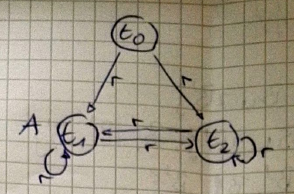
\includegraphics[width=3.71910in,height=2.33200in]{media/52typelim.png}

\paragraph{Beweis}

Zu zeigen: $\MI$ ist Modell von $C_{0}$ und $\MT$ *.

Behauptung: Für alle $C \in sub\left( C_{0},\MT \right)$ und alle
$t \in \Gamma_{i}$:
$$C \in t \Rightarrow t \in C^{\MI}$$

Daraus folgt:

\begin{enumerate}
\def\labelenumi{\arabic{enumi}.}
\item
  * Wegen $C_{0} \in t_{0}$ ist $t_{0} \in C_{0}^{\MI}$
\item
  Wegen $C_{T} \in t$ für alle $t \in \Gamma_{i}$ folgt
  $t \in C_{T}^{\MI}$. für alle $t \in \Gamma_{i}$ Also ist $\MI$ Modell von $\MT$.
\end{enumerate}

\textbf{I.A.} $C = A$. Folgt direkt aus Definition $\MI$.

$C = \neg A$. Nach Definition „Typ`` gilt $A \notin t$. Nach
Definition $\MI$ ist $t \notin A^{\MI}$.

\textbf{I.S.} Fallunterscheidung:

\begin{itemize}
\item
  $C = D \sqcap D^{'}$

Nach Definition „Typ`` ist $D \in t$ und $D^{'} \in t$. Nach
\textbf{I.V}.: $t \in D^{\MI}$ und $t \in \left( D^{'} \right)^{\MI}$.
Nach Semantik: $t \in \left( D \sqcap D^{'} \right)^{\MI}$.

\item
  $C = D \sqcup D^{'}$

Analog.

\item
  $C = \forall r.D$

Sei $\forall r.D \in t$ und $\left( t,t^{'} \right) \in r^{\MI}$. Nach
Definition $r^{\MI}$ muss $D \in t^{'}$ gelten. Nach \textbf{I.V}.:
$t^{'} \in D^{\MI}$, also $t \in \left( \forall r.D \right)^{\MI}$

\item
  $C = \exists r.D$

Sei $\exists r.D \in t$. Da $t \in \Gamma_{i}$ (also nicht
schlecht), gibt es $t^{'} \in \Gamma_{i}$ mit $D \in t^{'}$ und
$E \in t^{'}$ für alle $\forall r.E \in t$. Nach \textbf{I.V.} gilt
$t^{'} \in D^{\MI}$ und nach Definition von $r^{\MI}$ gilt
$\left( t,t^{'} \right) \in r^{\MI}$. Also
$t \in \left( \exists r.D \right)^{\MI}$
\end{itemize}

\textbf{Vollständigkeit}. 

Beweisskizze per Induktion über i.

Sei $C_{0}$ erfüllbar bzgl. $\MT$ und sei $\MI$ Modell von $\MT$ mit
$d_{0} \in C_{0}^{\MI}$. 

Sei $\Gamma = \left\{ t_{\MI}\left( d \right)\  \middle| \ d \in \Delta^{\MI} \right\}$.

Sei $\Gamma_{0},\ldots,\Gamma_{k}$ die von $\text {$\ALC$}\mathrm{-}\text{Elim}\left( C_{0},\MT \right)$ erzeugte Sequenz. 

Behauptung: $\Gamma \subseteq \Gamma_{i}$ für alle $i \geq 0$

Daraus folgt wegen $d_{0} \in C_{0}^{\MI}$, dass $C_{0} \in t_{i}\left( d_{0} \right) \in \Gamma \subseteq \Gamma_{k}$.

Also gibt $\text {$\ALC$}\mathrm{-}Elim(C_{0},\MT)$ „erfüllbar`` zurück.

I.A. $i = 0$. Einfach jedes Element von $\Gamma$ (semantisch Typ)
ist auch ein syntaktischer Typ.

I.S. Gelte $\Gamma \subseteq \Gamma_{i}$ (I.V.). Zu zeigen:
$\Gamma \subseteq \Gamma_{i + 1}$. 

Sei $t \in \Gamma$. Es genügt zu zeigen: $t$ ist nicht schlecht in $\Gamma_{i}$. 

Sei $\exists r.C \in t$ und $S = \left\{ C \right\} \cup \left\{ D \middle| \forall r.D \in T \right\}$.

Da $t \in \Gamma$, gibt es $d \in \Delta^{\MI}$ mit $t_{\MI}\left( d \right) = t_{0}$. 

Also gibt es nach Semantik $e \in \Delta^{\MI}$, $\left( d,e \right) \in r^{\MI}$, $e \in D^{\MI}$ für alle $D \in S$

$t's$ gilt also $S \subseteq t_{\MI}\left( e \right)$ und $t_{\MI}\left( e \right) \in \Gamma \subseteq \Gamma_{i}$. Es folgt:
$t$ nicht schlecht

\begin{theorem}
In $\ALC$ ist die Erfüllbarkeit von Konzepten bzgl. TBoxen entscheidbar in ExpTime.
\end{theorem}

\subsubsection{Zusammenhang mit Tableau-Algorithmen}

Offensichtliche Entsprechungen:

\begin{itemize}
  \item $\sqcap$-Regel, $\sqcup$-Regel, TBox-Regel finden sich wieder in der Definition eines Typs.
  \item $\exists$-Regel und $\forall$-Regel finden sich wieder in Def. von ``schlecht''.
  \item Freiheit von offensichtlichen Widersprüchen findet sich wieder in der Definition eines Typs
\end{itemize}

Unterschiede:

\begin{itemize}
  \item Tableau-Algorithmus benötigt im Worst Case dreifach exponentielle Laufzeit
  \item Typelimination benötigt im Best Case exponentielle Laufzeit
\end{itemize}

\subsection{Komplexität mit TBoxen, untere Schranke}\label{komplexituxe4t-mit-tboxen-untere-schranke}

Um die ExpTime-Härte zu zeigen, reduzieren wir auf ein spieltheoretisches Problem:

\subsubsection{ExpTime-Spiele}\label{exptime-spiele}

\begin{itemize}
\item
  Zwei Spieler spielen auf gegebener aussagenlogischen Formel
  $\varphi$
\item
  Jede Variable in $\varphi$ gehört entweder Spieler 1 oder Spieler 2
\item
  Das Spiel beginnt auf einer gegebenen Anfangsbelegung $\pi_{0}$ der
  Variablen
\item
  Spieler 1 beginnt, die Spieler wechseln sich ab
\item
  In jedem Zug ändert Spieler Wahrheitswert einer seiner Variablen; es
  ist erlaubt, zu passen
\item
  Spieler 1 gewinnt, wenn $\varphi$ jemals wahr wird (egal, welcher
  Spieler gezogen hat)
\item
  Spieler 2 gewinnt, wenn das Spiel unendlich weitergeht ohne dass
  $\varphi$ wahr wird
\end{itemize}

\begin{definition}{ExpTime-Spiele}

\begin{itemize}
\item
  \emph{Spiel}: Tupel
  $\left( \varphi,\ \Gamma_{1},\Gamma_{2},\pi_{0} \right)$ mit
  $\Gamma_{1},\Gamma_{2}$ Partitionierung der Variablen in
  $\varphi_{1}$ und $\pi_{0}$ Anfangsbelegung
\item
  \emph{Konfiguration}: Paar $(i,\pi)$ mit
  $i \in \left\{ 1,2 \right\}$ aktiver Spieler und $\pi$ Belegung
\item
  $\pi$ ist $j$-\emph{Variation} von $\pi'$
  $\left( j \in \left\{ 1,2 \right\} \right)$ wenn $\pi = \pi'$ oder
  $\pi$ und $\pi^{'}$ unterscheiden sich nur in einer Variablen
  $p \in \Gamma_{j}$
\end{itemize}
\end{definition}

„$\pi$ ist $j$-Variation von $\pi'$`` bedeutet: Spieler $j$ kann
$\pi$ in $\pi'$ transformieren (oder umgekehrt).

Das hier relevante Entscheidungsproblem bezieht sich auf \emph{Gewinnstrategien} für Spieler 2.

\subsubsection{Gewinnstrategie}\label{definition-5.8-gewinnstrategie}

Intuitiv:

\begin{itemize}
  \item eine Gewinnstrategie sagt Spieler 2 nach jedem möglichen Spielverlauf wie er spielen muss um zu gewinnen.
  \item wenn Spieler 2 eine Gewinnstrategie hat, so kann er das Spiel gewinnen
\end{itemize}

\begin{definition}{Gewinnstrategie}

Gewinnstrategie für Spieler 2 in Spiel
$\left( \varphi,\Gamma_{1},\Gamma_{2},\pi_{0} \right)$ ist unendlicher
knotenbeschrifteter Baum $(V,E,l)$, wobei $l$ jedem Knoten
$v \in V$ Konfiguration $l(v)$ zuweist so, dass

\begin{enumerate}
\def\labelenumi{\alph{enumi})}
\item
  Wurzel beschriftet mit $\left( 1,\pi_{0} \right)$
\item
  wenn $l\left( v \right) = (2,\pi)$, dann hat $v$ Nachfolger
  $v^{'}$ mit $l\left( v' \right) = \left( 1,\pi^{'} \right)$, wobei
  $\pi^{'}$ $2$-Variation von $\pi$
\item
  wenn $l\left( v \right) = (1,\pi)$, dann hat $v$ Nachfolger
  $v_{0},\ldots,v_{\left| \Gamma_{1} \right|}$ mit
  $l\left( v_{1} \right) = (2,\pi_{i})$ wobei
  $\pi_{0},\ldots,\pi_{\left| \Gamma_{1} \right|}$ alle existierenden
  $1$-Variationen von $\pi$
\item
  wenn $l\left( v \right) = (i,\pi)$, dann nicht
  $\pi \vDash \varphi$
\end{enumerate}
\end{definition}

\subsubsection{ExpTime-Spiele als Entscheidungsproblem}

\begin{definition}

\emph{Spiel\textsubscript{1}} ist das folgende Problem: Gegeben Spiel
$\left( \varphi,\Gamma_{1},\Gamma_{2},\pi_{1} \right)$, entscheide ob
Spieler 2 eine Gewinnstrategie hat.
\end{definition}

\begin{theorem}
Spiel\textsubscript{1} ist ExpTime-Vollständig
\end{theorem}

Wir wollen nun die ExpTime-Härte von Erfüllbarkeit in $\ALC$ bzgl. TBoxen auf Spiel\textsubscript{1} reduzieren

\subsubsection{Reduktion}\label{reduktion}

Reduziere Spiel\textsubscript{1}: Gegeben Spiel
$\left( \varphi,\Gamma_{1},\Gamma_{2},\pi_{0} \right)$, konstruiere in
Polynomialzeit Konzept $C_{S}$ und TBox $\MT_{S}$ so, dass: 

\begin{lemma}Spieler 2 hat Gewinnstrategie in $S$ gdw. $C_{S}$ erfüllbar bzgl. $\MT_{S}$.\end{lemma}

Idee: (Baum)-Modelle von $C_S$ und $\MT_S$ kodieren Gewinnstrategien.

Beweisskizze:

Details der Reduktion:


\includegraphics[width=3.71910in,height=2.33200in]{media/5red1.png}


\includegraphics[width=3.71910in,height=2.33200in]{media/5red2.png}


\includegraphics[width=3.71910in,height=2.33200in]{media/5red3.png}

Setze $C_S = W$ 

\begin{itemize}
\item
  Hinrichtung: Erzeuge aus der Gewinnstrategie Interpretation und zeige, dass diese Modell ist.
\item
  Rückrichtung: Nimm an es gibt Baummodell und erzeuge daraus
  Gewinnstrategie.
\end{itemize}

\begin{theorem}
In $\ALC$ ist die Erfüllbarkeit von TBoxen ExpTime-hart.
\end{theorem}

Daraus ergibt sich zusammen mit \protect\hyperlink{theorem-5.6}{Theorem 5.6} ExpTime-Vollständigkeit.

\subsection{Komplexität ohne TBoxen obere
Schranke}\label{komplexituxe4t-ohne-tboxen-obere-schranke}

\subsubsection{Obere Schranke}

Wir wollen zeigen:

\begin{theorem}
In $\ALC$ ist die Erfüllbarkeit von Konzepten (ohne TBoxen)
PSpace-Vollständig.
\end{theorem}

Mit Lemma 2.8 sind dann auch Subsumtion und Äquivalenz PSpace-vollständig.

\subsubsection{ALC-Worlds}\label{alc-worlds}

Wenn $C$ erfüllbar, dann hat $C$ ein Baummodell (Theorem 3.4). Ohne TBox ist dessen Tiefe mit $\left| C \right|$ beschränkt. 

In PSpace:

\begin{itemize}
\item
  Ein linear Tiefer Baum ist exponentiell groß
\item
  Gesamtes Modell im Speicher: nicht PSpace
\item
  Stattdessen Prüfe Existenz des Baumes mittels Tiefensuche; halte zu
  jeder Zeit nur einen Pfad des Baumes im Speicher
\end{itemize}

\begin{theorem}
PSpace $=$ NPSpace
\end{theorem}

\begin{definition}{$i$-Konzepte}

Für $i \geq 0$ ist die Menge der $i$-Konzepte definiert als:
$$sub_{i} := \left( C_{0} \right) \left\{ C \in sub\left( C_{0} \right)\  \middle| \text{\ rd}\left( C \right) \leq i \right\}$$
\end{definition}

\begin{definition}{i-Typ}

Sei $i \geq 0$. $\MI$-Typ für $C_{0}$ ist Teilmenge
$t \subseteq sub_{i}\left( C_{0} \right)$ so, dass

\begin{enumerate}
\def\labelenumi{\arabic{enumi}.}
\item
  $A \in t$ gdw. $\neg A \notin t$ für alle
  $\neg A \in sub_{i}\left( C_{0} \right)$
\item
  $C \sqcap D \in t$ gdw. $C \in t$ und $D \in t$ für alle
  $C \sqcap D \in sub_{i}\left( C_{0} \right)$
\item
  $C \sqcup D \in t$ gdw. $C \in t$ oder $D \in t$ für alle
  $C \sqcup D \in sub_{i}\left( C_{0} \right)$
\end{enumerate}
\end{definition}

\paragraph{ALC-Worlds}\label{alc-worlds-1}

Rekursion über $\MI$-Typen.

\begin{proposition}
ALC-Worlds($C_{0}$) terminiert und benötigt polynomiellen Platz (in $|C_0|$).
\end{proposition}

Beweisskizze. Stelle als Rekursionsbaum dar. Verzweigungsgrad beschränkt durch Anzahl der $\exists$. Tiefe Beschränkt durch $rd(C_{0})$. Der Rekursionsstack hat höchstens Tiefe $\left| C_{0} \right|$ und der Platzbedarf pro Aufruf ist polynomiell.

\subsubsection{Korrektheit und Vollständigkeit}\label{proposition-5.18}

\begin{proposition}
$\ALC$-Worlds($C_0$) = true gdw. $C_0$ erfüllbar
\end{proposition}

Korrektheitsbeweis per Induktion über $C_{0}$:

Zunächst definieren wir eine Interpretation $\MI$. Für jeden Knoten $v \in V_0 \setminus \{v_0\}$ sei $\sigma (v)$ der Rollenname $r$ des Konzeptes $\exists r.C$, für das der Aufruf $v$ gemacht wurde.

Definiere $\MI$ nun wie folgt:

\begin{itemize}
  \item $\Delta^{\MI} = V$
  \item $r^{\MI} = \{(v,v')\in E | \sigma (v') = r\}$
  \item $A^{\MI} = \{v | A \in p_1(v)\}$
\end{itemize}

($p_1(v)$ = 1. Parameter in $l(v)$)

Behauptung: Für alle $v \in V$ und $C \in sub(C_0)$ gilt $$C \in p_1(v)\ impliziert v \in C^{\MI}$$

Da $C_0 \in p_1(v_0)$ ist auch $v_0 \in C_0^{\MI}$; also ist $\MI$ ein Modell von $C_0$.

\textbf{T5.9a}

\textbf{I.A.} $C = A$. Folgt direkt aus Definition $\MI$.

$C = \neg A$. Da der Lauf erfolgreich ist, ist
$p_{1}\left( v \right)$ Typ für $C_{0}$. Nach Definition „Typ`` gilt
$A \notin p_{1}\left( v \right)$. Nach Definition $\MI$ ist
$v \notin A^{\MI}$.

\textbf{I.S.} Fallunterscheidung:

\begin{itemize}
\item
  $C = D \sqcap D^{'}$
\end{itemize}

Nach Definition „Typ`` ist $D \in p_{1}\left( v \right)$ und
$D^{'} \in p_{1}\left( v \right)$. Nach \textbf{I.V}.: $v \in D^{\MI}$
und $v \in \left( D^{'} \right)^{\MI}$. Nach Semantik:
$v \in \left( D \sqcap D^{'} \right)^{\MI}$.

\begin{itemize}
\item
  $C = D \sqcup D^{'}$
\end{itemize}

Analog.

\begin{itemize}
\item
  $C = \forall r.D$
\end{itemize}

Sei $\left( v,v^{'} \right) \in r^{\MI}$. Dann ist
$\left( v,v^{'} \right) \in E$ und $\sigma\left( v^{'} \right) = r$.
Wegen $\forall r.D \in p_{1}(v)$ ist auch
$D \in p_{1}\left( v^{'} \right)$. Nach I.V. gilt $v^{'} \in D$.
Also $v \in \left( \forall r.D \right)^{\MI}$

\begin{itemize}
\item
  $C = \exists r.D$
\end{itemize}

Ähnlich

\textbf{Beweis der Vollständigkeit}

Sei $C_0$ erfüllbar und $\MI$ ein Modell von $C_0$ und $d_0 \in C_0^{\MI.}$

Beweisidee:

Verwenden $\MI$, um die nichtdeterministischen Entscheidungen von $\ALC$-Worlds($C_0$) zu einem erfolgreichen Lauf zu ``lenken''.

\begin{theorem}
In $\ALC$ ist die Erfüllbarkeit von Konzepten in PSpace.
\end{theorem}

\subsection{Komplexität ohne TBoxen untere
Schranke}\label{komplexituxe4t-ohne-tboxen-untere-schranke}

\begin{definition}{PSpace-Spiel}

\begin{itemize}
\item
  \emph{Spiel}: Aussagenlogische Formel $\varphi$ mit Variablen
  $p_{1},\ldots,p_{n}$, $n$ gradzahlig
\item
  \emph{Konfiguration}: Wort $\pi \in \left\{ 0,1 \right\}*$
\end{itemize}
\end{definition}

\begin{definition}{Gewinnstrategie}

Gewinnstrategie für Spieler 1 in Spiel $\varphi$ ist endlicher
knotenbeschrifteter Baum $(V,E,L)$, wobei $l$ jedem Koten
$v \in V$ Konfiguration $l(v)$ zuweist, sodass
\end{definition}

\begin{enumerate}
\def\labelenumi{\alph{enumi})}
\item
  Wurzel beschriftet mit $\varepsilon$ (leere Konfiguration)
\item
  wenn $l\left( v \right) = w$ mit $\left| w \right|$ gerade und
  $\left| w \right| < n$ (Also Spieler 1 am Zug), dann hat $v$
  Nachfolger $v^{'}$ mit $l\left( v^{'} \right) \in \{ w0,w1\}$
\item
  wenn $l\left( v \right) = w$ mit \textbar{}w\textbar{} ungerade
  (also Spieler 2 am Zug), dann hat $v$ Nachfolger $v^{'}$ und
  $v''$mit $l\left( v^{'} \right) = w0$ und
  $l\left( v^{''} \right) = w1$
\item
  wenn $l\left( v \right) = w$ mit $\left| w \right| = n$, dann
  $w \vDash \varphi$
\end{enumerate}

\subsubsection{Theorem 5.25}\label{theorem-5.25}

In $\ALC$ ist die Erfüllbarkeit von Konzepten bzgl. leerer TBoxen
PSpace-Hart.

Beweisskizze. Konstruiere Konzept $C_{\varphi}$, so dass Spieler 1 hat
Gewinnstrategie in $\varphi$ gdw. $C_{\varphi}$ erfüllbar.

\subsection{Unentscheidbare
Erweiterungen}\label{unentscheidbare-erweiterungen}

\subsection{Konkrete Bereiche}\label{konkrete-bereiche}

Ein \emph{Konkreter Bereich} ist ein Paar $B = (\Delta^{B},\Phi^{B})$
wobei

\begin{itemize}
\item
  $\Delta^{B}$ eine Menge von \emph{Werten} ist und
\item
  $\Phi^{B}$ eine Menge von \emph{Prädikaten}
\end{itemize}

sodass jedes $P \in \Phi^{B}$ mit einer Stelligkeit $n \geq 0$
ausgestattet ist und mit einer Extension
$P^{B} \subseteq \left( \Delta^{B} \right)^{n}$.

\subsubsection{Definition 5.27 (ALCB
Syntax)}\label{definition-5.27-alcb-syntax}

Sei $B$ ein konkreter Bereich. Mit ALC($B$) bezeichnen wir die
Erweiterung von $\ALC$ um $B$, d.h. um

\begin{itemize}
\item
  \emph{Featurenamen} (eine zusätzliche Art von Rolle) und
\item
  die Konstruktoren $\exists R_{1},\ldots,\ R_{n}\text{.P}$ und
  $\forall R_{1},\ldots,R_{n}\text{.P}$
\end{itemize}

wobei $P \in \Phi^{B}$ $n$-Stellig ist und die $R_{i}$
\emph{Rollenkomposition} der Form $r_{1};\ldots;r_{k};f$ sind mit
$r_{j}$ Rollenname und $f$ Featurename.

\subsubsection{Definition 5.28 (ALCB
Semantik)}\label{definition-5.28-alcb-semantik}

Eine Interpretation $\MI$ ordnet nun zusätzlich zu jedem Featurenamen
$f$ eine Funktion $f^{\MI}:\Delta^{\MI} \rightarrow \Delta^{B}$ zu. Für
jede Rollenkomposition $r = r_{1};\ldots r_{k};f$ bezeichnet $R^{\MI}$
die Komposition der Interpretationen:
$R^{\MI} = r_{1}^{\MI} \circ \ldots \circ r_{k}^{\MI} \circ f$

Die Semantik der zusätzlichen Konstruktoren ist nun:

\[\left( \exists R_{1},\ldots,\ R_{k}\text{.P} \right)^{\MI} = \left\{ d \in \Delta^{\MI}\ |\ \exists d_{1},\ldots,d_{k}:\left( d,d_{i} \right) \in R_{i}^{\MI}\ \mathrm{fur}\ 1 \leq i \leq k\ \mathrm{\text{und}}\ \left( d_{1},\ldots,\ d_{k} \right) \in P^{B} \right\}\]

\[\left( \forall R_{1},\ldots,\ R_{k}\text{.P} \right)^{\MI} = \left\{ d \in \Delta^{\MI}\ |\ \forall d_{1},\ldots,d_{k}:\left( d,d_{i} \right) \in R_{i}^{\MI}\ \mathrm{fur}\ 1 \leq i \leq k\ \mathrm{\text{impliziert}}\ \left( d_{1},\ldots,\ d_{k} \right) \in P^{B} \right\}\]

\subsubsection{2-Registermaschinen}\label{registermaschinen}

\begin{itemize}
\item
  Endlich viele Zustände
\item
  Zwei Register mit Werten aus $\mathbb{N}$
\item
  Instruktionen um

  \begin{itemize}
  \item
    Register zu inkrementieren
  \item
    Register auf null zu testen und bei Wert $\neq 0$ zu
    dekrementieren. Der Folgezustand hängt davon ab, ob das Register
    $0$ war.
  \end{itemize}
\end{itemize}

\subsubsection{Definition 5.30}\label{definition-5.30}

(Deterministische) \emph{2-Registermaschine} (2RM) ist Paar
$M = \left( Q,P \right)$ mit
$Q = \left\{ q_{0},\ldots,\ q_{l} \right\}$ Menge von \emph{Zuständen}
und $P = I_{0},\ldots,I_{l - 1}$ \emph{Instruktionsfolge}. Per
Definition ist $q_{0}$ Startzustand, $q_{l}$ Stoppzustand. Jede
Instruktion ist $I_{i}$ hat eine der folgenden Formen:

\begin{itemize}
\item
  $I_{i} = + (p,q_{1})$ mit $p \in \left\{ 1,2 \right\}$
  \emph{Register} und $q_{j}$ Folgezustand: Inkrementierunsanweisung
\item
  $I_{i} = - (p,q_{j},q_{k})$ mit $p \in \left\{ 1,2 \right\}$
  Register und $q_{j},q_{k}$ Folgezustände: Dekrementierungsanweisung
  mit Folgezustand $q_{j}$, wenn Register $p$ den Wert $0$ enthält
  und $q_{k}$ sonst.
\end{itemize}

\subsubsection{Definition 5.31}\label{definition-5.31}

Konfiguration und Konfigurationsübergänge
$\left( q,m,n \right) \vdash_{M}(q^{'},m',n^{'})$. Berechnung als
eindeutige längste Konfigurationsfolge.

\subsubsection{Theorem 5.29}\label{theorem-5.29}

Das Erfüllbarkeitsproblem in $ALC(B_{1})$ ist unentscheidbar.

\begin{itemize}
\item
  $\Delta^{B_{1}}\mathbb{= N}$
\item
  $\Phi^{B_{1}} = \left\{ =_{0}, = , +_{1} \right\}$, wobei $=_{0}$
  einstellig, die anderen Zweistellig.
\end{itemize}

Beweisskizze. Gegeben 2RM $M$,
konstuiere$\text {$\ALC$}\left( B_{1} \right)$-TBox $T_{M}$ und wähle
einen Konzeptnamen $J$ sodass: $M$ hält auf $\left( 0,0 \right)$
gdw. $J$ unerfüllbar bzgl. $T_{M}$. Zeige dies jeweils für
Hinrichtung und Rückrichtung per Kontraposition. \textbf{Wo kommen i und
j her?}
	\newpage

	\section{Effiziente Beschreibungslogiken}
	
\subsection{EL}\label{el}

Ein EL-Konzept ist ein ALC-Konzept, in dem nur die Konstruktoren
$\top,\ $ $\sqcap$ und $\exists r.C$ verwendet werden.

\subsection{Simulation}\label{simulation}

Simulation ist gerichtete Bisimulation.
$\left( I_{1},d_{1} \right) \precsim \left( I_{2},d_{2} \right)$: es
gibt Simulation $p$ von $I_{1}$ nach $I_{2}$ mit
$d_{1}\text{\ p\ }d_{2}$.

\hypertarget{lemma-6.3}{\subsubsection{Lemma 6.3}\label{lemma-6.3}}

Seien $I_{1},I_{2}$ Interpretationen, $d_{1} \in \Delta^{I_{1}}$ und
$d_{2} \in \Delta^{I_{2}}$. Wenn
$\left( I_{1},d_{1} \right) \precsim \left( I_{2},d_{2} \right)$, dann
gilt für alle EL-Konzepte $C$: $d_{1} \in C^{I_{1}}$ impliziert
$d_{2} \in C^{I_{2}}$.

Beweisskizze per Induktion über die Struktur von $C$. Sei $\rho$
eine Simulation zwischen $I_{1}$ und $I_{2}$ mit
$d_{1}\text{\ $\rho$}\text{\ d}_{2}$.

\textbf{I.A.} $C = A$ ist Konzeptname. Nach Bedingung 1. der
Bisimulation gilt $d_{1} \in A^{I_{1}}$ impliziert
$d_{2} \in A^{I_{2}}$.

\textbf{I.S.} Unterscheide Fälle gemäß dem äußersten Konstrukt von
$C$.

\begin{enumerate}
\def\labelenumi{\arabic{enumi}.}
\item
  $C = D_{1} \sqcap D_{2}$
\end{enumerate}

\begin{quote}
$d_{1} \in C^{I_{1}}$ gdw. $d_{1} \in D_{1}^{I_{1}}$und
$d_{1} \in D_{2}^{I_{1}}$ (Semantik) impliziert.
$d_{2} \in D_{1}^{I_{2}}$ und $d_{2} \in D_{2}^{I_{2}}$ (I.V.) gdw.
$d_{2} \in C^{I_{2}}$ (Semantik)
\end{quote}

\begin{enumerate}
\def\labelenumi{\arabic{enumi}.}
\item
  $C = \exists r.D$
\end{enumerate}

\begin{quote}
Hinrichtung und Rückrichtung analog über Semantik, 2. Bedingung der
Simulation, I.V., Semantik.
\end{quote}

\subsubsection{Lemma 6.4}\label{lemma-6.4}

Bisimulation und wechselseitige Simulation sind nicht dasselbe.

Beweisskizze: Zeige Wechselseitige Simulation, die keine Biosimulation
ist:

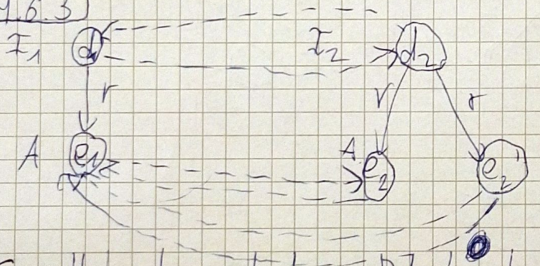
\includegraphics[width=3.71910in,height=1.83200in]{media/image1.png}

\subsubsection{Lemma 6.6}\label{lemma-6.6}

Jedes EL-Konzept ist erfüllbar bzgl. jeder TBox.

Beweisskizze per Induktion über die Struktur von $C$:


\includegraphics[width=2.50460in,height=1.15200in]{media/image2.png}

\subsection{Subsumtion ohne TBox}\label{subsumtion-ohne-tbox}

Eine Subsumption $C \sqsubseteq D$ gilt in EL im Prinzip gdw mann
$D$ syntaktisch in $C$ „wiederfindet``. Werden Konzepte als
Baummodell dargestellt entspricht „Wiederfinden`` Simulation von
$D$-Baum in $C$-Baum (also Teilgraphenproblem).

\subsubsection{Definition kanonisches
Modell}\label{definition-kanonisches-modell}

Baue aus dem gegebenen Konzept $C$ intuitiv Baummodell.

\hypertarget{lemma-6.8}{\subsubsection{Lemma 6.8}\label{lemma-6.8}}

Für alle EL-Konzepte $C$ gilt: Die Interpretation $I_{C}$ ist Modell
von $C$ mit $d_{w} \in C^{I_{C}}$.

Beweisskizze per Induktion über die Struktur von $C$.

\hypertarget{lemma-6.9}{\subsubsection{Lemma 6.9}\label{lemma-6.9}}

Für alle EL-Konzepte $C$, Interpretation $I$ und
$e \in \Delta^{I}$ gilt: $e \in C^{I}$ gdw.
$\left( I_{C},d_{w} \right) \precsim \left( I,e \right)$.

Beweisskizze.

\begin{itemize}
\item
  Hinrichtung per Induktion über $C$. Schau jeweils Simulation nach
  I.V. an und ergänze diese.
\item
  Rückrichtung. Angenommen
  $\left( I_{C},d_{w} \right) \precsim \left( I,e \right)$.
  \protect\hyperlink{lemma-6.8}{Lemma 6.8} liefert
  $d_{w} \in C^{I_{C}}$. Nach \protect\hyperlink{lemma-6.3}{Theorem
  6.3} ist $e \in C^{I}$.
\end{itemize}

\subsubsection{Lemma 6.10}\label{lemma-6.10}

Für alle EL-Konzepte $C$, $D$ gilt: $C \sqsubseteq D$ gdw.
$\left( I_{D},d_{w} \right) \precsim \left( I_{C},d_{w} \right)$

Beweisskizze.

\begin{itemize}
\item
  Hinrichtung: Betrachte kanonisches Modell $I_{C}$ von $C$. Wegen
  Lemma 6.8 gibt es $d_{w} \in C^{I_{C}}$. Mit $C \sqsubseteq D$
  folgt $d_{W} \in D^{I_{C}}$. Mit \protect\hyperlink{lemma-6.9}{Lemma
  6.9} folgt für $D,\ I_{C},d$ dass $d_{w} \in D^{I_{C}}$ gdw.
  $\left( I_{D},d_{w} \right) \precsim \left( I_{C},d_{w} \right)$.
\item
  Rückrichtung. Angenommen
  $\left( I_{D},d_{w} \right) \precsim \left( I_{C},d_{w} \right)$.
  Betrachte beliebige Interpretation $I$ und $d \in C^{I}$. Zu
  zeigen: $d \in D^{I}$. Wegen $d \in C^{I}$ und
  \protect\hyperlink{lemma-6.9}{Lemma 6.9} gilt
  $\left( I_{C},d_{w} \right) \precsim \left( I,d \right)$. Verkette
  die Simulationen so dass
  $\left( I_{D},d_{w} \right) \precsim \left( I,d \right)$. Mit
  \protect\hyperlink{lemma-6.9}{Lemma 6.9} folgt
  $d_{w} \in D^{I_{C}}$.
\end{itemize}

\subsubsection{Theorem 6.11}\label{theorem-6.11}

Subsumtion in EL kann in polynomieller Zeit entschieden werden:

\begin{itemize}
\item
  Konstruiere $I_{C}$ und $I_{D}$ in polynomieller Zeit.
\item
  Überprüfe in polynomieller Zeit, ob
  $\left( I_{D},d_{w} \right) \precsim \left( I_{C},d_{w} \right)$

  \begin{itemize}
  \item
    Berechne maximale Simulation $\varsigma$
  \item
    Teste ob $\left( d_{w},d_{W} \right) \in \varsigma$
  \item
    \textbf{Sascha}
  \end{itemize}
\end{itemize}

\subsection{Subsumption mit TBox}\label{subsumption-mit-tbox}

\subsubsection{Lemma 6.12}\label{lemma-6.12}

Seien $C,D$ zwei beliebige $\text{EL}$-Konzepte und $T$ eine
EL-TBox. Sei weiterhin
$T^{'} = T \cup \left\{ A_{C} \sqsubseteq C,D \sqsubseteq A_{D} \right\}$.
mit Konzeptnamen $A_{C},A_{D}$, die nicht in $C,D,T$ vorkommen. Dann
gilt; $T \vDash C \sqsubseteq D$ gdw
$T^{'} \vDash A_{C} \sqsubseteq A_{D}$.

\subsubsection{ Normalform}\label{normalform}

Eine TBox ist in \emph{Normalform}, wenn sie nur Inklusionen folgender
Form enthält:

$A_{1} \sqcap \ldots \sqcap A_{n} \sqsubseteq A$
$A \sqsubseteq \exists r.A_{1}$ $\exists r.A \sqsubseteq A_{1}$

\subsubsection{Lemma 6.14}\label{lemma-6.14}

Jede EL-TBox $T$ kann in polynomieller Zeit in eine TBox $T^{'}$ in
Normalform gewandelt werden, so dass für alle Konzeptnamen $A,B$ in
$T$ gilt: $T \vDash A \sqsubseteq B$ gdw
$T \vDash A \sqsubseteq B$. Dann ist $T'$ \emph{konservative
Erweiterung} von $T$.

\subsubsection{Lemma 6.14}\label{lemma-6.14-1}

Jede EL-TBox $T$ kann durch linear viele Regelanwendungen in TBox in
Normalform transformiert werden, die konservative Erweiterung von $T$
ist.

Die Regeln fügen jeweils Zwischenkonzepte ein.

Beweisskizze: Grad der Abnormalität definieren und zeigen, dass

\begin{enumerate}
\def\labelenumi{\arabic{enumi}.}
\item
  Der Grad ist beschränkt durch $\left| T \right|$
\item
  Jede Regelanwendung verringert den Grad
\item
  TBoxen vom Grad $0$ sind in Normalform
\end{enumerate}

\subsubsection{Algorithmus}\label{algorithmus}

Wende Regeln erschöpfend an um alle Subsumptionen zu berechnen:

$\frac{\ }{A \sqsubseteq A}$ (Wenn $A$ in $T$ vorkommt)
$\frac{\ }{A \sqsubseteq \top}$ (Wenn $A$ in $T$ vorkommt)

$\frac{A \sqsubseteq A_{1},\ldots,A \sqsubseteq A_{n},A_{1} \sqcap \ldots \sqcap A_{n} \sqsubseteq B}{A \sqsubseteq B}$
$\frac{A \sqsubseteq \exists r.A_{1},\ A_{1} \sqsubseteq B_{1},\exists r.B_{1} \sqsubseteq B}{A \sqsubseteq B}$

\textbf{Wo gehört das x hin Vorlesung 17?}

Für eine EL-TBox $T$ sei $T*$ das Ergebnis erschöpfender
Regelanwendungen, die \emph{Saturierung}.

\subsubsection{Theorem 6.16 }\label{theorem-6.16}

Für alle Konzeptnamen $A,B$ in $T$ gilt:
$T \vDash A \sqsubseteq B$ gdw $A \sqsubseteq B \in T*$

\paragraph{Terminierung}\label{terminierung-1}

Beweisskizze. Jede Regelanwendung erzeugt eine neue Konzeptinklusion
$A \sqsubseteq B$, wobei $A,B$ Konzeptnamen aus $T$. Es gibt nur
endlich viele solcher Inklusionen.

\paragraph{Korrektheit}\label{korrektheit-1}

Beweisskizze. Sei $T = T_{0},\ \ldots,(T_{n} = T*)$ die durch
Regelanwendungen erzeugte Folge von TBoxen. Es genügt zu zeigen:
$T_{i} \vDash T_{i + 1}$. Zeige dies durch Vorbedingung der
Regelanwendung und der Semantik.

\paragraph{Vollständigkeit}\label{vollstuxe4ndigkeit-1}

\subparagraph{Kanonische
Interpretation}\label{kanonische-interpretation}

Die Kanonische Interpretation $I$ ist:

\begin{itemize}
\item
  $\Delta^{I} = \left\{ d_{A}\ |\ A\ \mathrm{\text{Konzeptname\ in\ T}}* \right\} \cup \left\{ d_{\top} \right\}$
\item
  $A^{I} = \left\{ d_{\text{B\ }} \middle| \ B \sqsubseteq A \in T* \right\}$
\item
  $r^{I} = \left\{ \left( d_{A},d_{B} \right)\  \middle| \ A \sqsubseteq A^{'} \in T*\ \mathrm{\text{und}}\ A^{'} \sqsubseteq \exists r.B \in T*,\ A^{'}\ \mathrm{\text{Konzeptname}} \right\}$
\end{itemize}

Erklärung: Konstruiere Intuitiv Modell aus allen Konzeptnamen.

\hypertarget{lemma-6.18}{\subparagraph{Lemma 6.18}\label{lemma-6.18}}

Die kanonische Interpretation ist ein Model von $T*$.

Beweis: Zeige, dass alle Inklusionen in $T*$ von $I$ erfüllt werden.
Verwende die Inklusionen in Normalform. Überlege dazu, was aus den
Inklusionen mithilfe der Definition gefolgert werden kann.

\subparagraph{Vollständigkeit}\label{vollstuxe4ndigkeit-2}

Angenommen $A \sqsubseteq B \notin T*$. Betrachte Element $d_{A}$
der kanonischen Interpretation $I$. Wegen R1:
$A \sqsubseteq A \in T*$, also nach Def. $I$: $d_{A} \in A^{I}$.
Def. von $I$ und $A \sqsubseteq B \notin T*$ liefern
$d_{A} \notin B$. Da $I$ Modell von $T*$
(\protect\hyperlink{lemma-6.18}{Lemma 6.18}), und damit von $T$, folgt
nicht $T \vDash A \sqsubseteq B$.

\subsection{Erweiterungen von EL}\label{erweiterungen-von-el}

\hypertarget{el-mit-disjunktion-und-bottom}{\subsubsection{EL mit
Disjunktion und Bottom}\label{el-mit-disjunktion-und-bottom}}

Erfüllbarkeit in $\text{ELU}_{\bot}$ (mit Disjunktion) ist
ExpTime-Vollständig.

Beweisskizze per Reduktion von Erfüllbarkeit von Konzeptname $A$ bzgl.
ALC-TBox $T$:

\begin{enumerate}
\def\labelenumi{\arabic{enumi}.}
\item
  Ersetze Werterestriktion in $T$ durch Existenzrestriktion.
\item
  Bringe $T$ in Negationsnormalform.
\item
  Ersetze $\neg X$ durch $\overset{\overline{}}{X}$ mit
  $\top \sqsubseteq X \sqcup \overset{\overline{}}{X}$ und
  $X \sqcap \overset{\overline{}}{X} \sqsubseteq \bot$
\end{enumerate}

\subsubsection{ELU (mit Disjunktion)}\label{elu-mit-disjunktion}

Erfüllbarkeit in ELU ist ExpTime-Vollständig.

Beweisskizze per Reduktion von
\protect\hyperlink{el-mit-disjunktion-und-bottom}{6.5.1}. Ersetzte
$\bot$ durch $L$ mit $\exists r.L \sqsubseteq L$ für alle
Rollennamen $r$ in $T$.

	\newpage

	\section{ABoxen und Anfragebeantwortung}
	\subsection{Grundlagen}

\subsubsection{Ziel}

TBoxen repräsentieren nur allgemeines, begriffliches Wissen. Um konkrete Situationen zu repräsentieren, braucht man Instanzdaten.

Daher wird in diesem Kapitel ein Formalismus für Instanzdaten (ABox) eingeführt, die Schlussfolgerungsprobleme betrachtet, um mit Instanzdaten zu arbeiten und Anfragebeantwortung mit Datenbanksystemen und Ontologien (Query Rewriting) behandelt.

\subsubsection{ABoxen-Syntax}

\begin{definition}{ABoxen, Syntax}

\begin{itemize}
	\item Eine \emph{Konzerptassertion} hat die Form $A(a)$, $A$ Konzeptname.
	\item Eine Rollenassertion hat die Form $r(a,b)$, $r$ Rollenname.
\end{itemize}

Eine ABox ist eine endlcihe Menge von (Konzept- und Rollen-)assertionen
\end{definition}

\textbf{T7.1}

Eine Beispiel ABox:

\begin{itemize}
	\item $StudentIn(hanna)$
	\item $Person(klaus)$
	\item $bekanntMit(hanna,klaus)$
	\item $TheorieVL(blVl)$
	\item $hoert(hanna, blVl)$
	\item $VL(logikVL)$
\end{itemize}

Mit $Ind(\MA)$ bezeichnen wir die Menge der in $\MA$ verwendeten Individuen.

\subsubsection{ABoxen-Semantik}

\begin{definition}{Aboxen, Semantik}

Interpretation $\MI$

\begin{itemize}
	\item \emph{erfüllt} $A(a)$, wenn $a \in A^{\MI}$;
	\item \emph{erüfllt} $r(a,b)$, wenn $(a,b) \in r^{\MI}$.
\end{itemize}

$\MI$ ist \emph{Modell} von $\MA$, wenn $\MI$ alle Assertionen in $\MA$ erfüllt.
\end{definition}

\textbf{Beachte:}

Modell $\MI$ darf zusätzlich Assertionen wahr machen, die in $\MA$ \emph{nicht} vorkommen.

Das in ABoxen repräsentierte Wissen ist also unvollständiges Wissen.

\textbf{T7.1cont}

Eine Interpretation $\MI$:

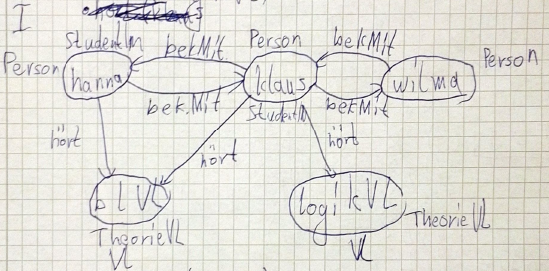
\includegraphics[width=5.21910in,height=2.83200in]{media/71abox.png}

\subsubsection{Wissensbasen}

\begin{definition}

\emph{Wissensbasis (WB)} $\MK = (\MT , \MA)$ besteht aus TBox $\MT$ und ABox $\MA$. Interpretation $\MI$ ist Modell von $\MK$, wenn $\MI$ Modell von $\MT$ und von $\MA$.
\end{definition}

In vielen Anwendungen werden $\MT$ nur einmal erstellt und ändert sich danach üblicherweise nicht mehr, aber $\MA$ ändert sich häufig.

\subsubsection{Grundlegende Schlussfolgerungsprobleme}

\begin{definition}{Konsistenz, Instanz}

Sei $\MK$ Wissensbasis, $A(a)$ Konzeptasertion. Dann ist

\begin{itemize}
	\item $\MK$ \emph{konsistenz}, wenn $\MK$ Modell hat;
	\item $a$ eine Instanz von $A$ bzgl. $\MK$, wenn jedes Modell von $\MK$ auch $A(a)$ erfüllt. Wir schreiben dann $\MK \models A(a)$.
\end{itemize}
\end{definition}

\textbf{T7.2}

$\MK = (\MT, \MA)$

$\MT = \{StudentIn \equiv Person \sqcap \exists hoert.Vl, TheorieVL \sqsubseteq VL\}$

(1) $\MK$ ist konsistent. $\MI$ aus T7.1 erfüllt $(\MT,\MA)$

(2) $\MK' \models StudentIn(klaus)$ mit $\MK' = (\MT, \MA')$ und 

sei $\MA' = \MA \cup \{hoert(klaus,blVL)\}$.

Sei $\MI$ Modell von $\MK'$. 

$\MA'$ liefert $klaus \in Person^{\MI}$, $(klaus,blVL) \in hoert^{\MI}$ und $blVL \in TheorieVL^{\MI}$.

KI2 von $\MT$ liefert $blVL \in VL^{\MI}$

KI1 von $\MT$ liefert $klaus \in StudentIn^{\MI}$

(3) $\MK \not\models TheorieVL(logikVL)$

    ist zwar in $\MI$ aus T7.1 erfüllt, aber setzt man $TheorieVL^{\MI} = \{blVL \}$ so hat man immer noch ein Modell von $\MA,\MT$ 

\textbf{Konsistenzproblem}:

Gegeben $\MK$, entscheide ob $\MK$ konsistent ist.

\textbf{Instanzproblem}:

Gegeben $\MK$ und $A(a)$, entscheide ob $\MK \models A(a)$.

\subsubsection{Reduktionen}

Konsistenz- und (Nicht-)Instanzproblem wechselseitig polynomiell reduzierbar:

\begin{lemma} 

\begin{itemize}
	\item $\MK$ ist konsistent gdw. $\MK \not\models A(a)$, $A$ neuer Konzeptname
	\item $(\MT, \MA) \models A(a)$ gdw. $(\MT \cup \{\MT \cup \{\overline{A} \equiv \neg A\}\})$ inkosistent
\end{itemize}
\end{lemma}

\textbf{T7.3}

(1) $\MK$ konsistenz

gdw. $\MK$ hat Modell

gdw. $\MK$ hat Modell $\MI$ mit $a \not\in A^{\MI}$

gdw. $\MK \not\models A(a)$

(2) $(\MT, \MA) \not\models A(a)$

gdw. es gibt Modell $\MI$ von $(\MT, \MA)$ mit $a \not\in A^{\MI}$ (Def. 7.4)

gdw. es gibt Modell $\MI$ von $(\MT \cup \{\overline{A} \equiv \neg A\}, \MA)$ mit $a \not\in A^{\MI}$

gdw. es gibt Modell $\MI$ von $(\MT \cup \{\overline{A} \equiv \neg A\}, \MA \cup \{\overline{A}(a)\})$

gdw. $(\MT \cup \{\overline{A} \equiv \neg A\}, \MA \cup \{\overline{A}(a)\})$ konsistent

\textbf{T7.2cont}

Instanzanfragen z.B:

StudentIn

Vl

TheorieVl

\textbf{T7.4}

$\MI$ aus Bsp. 7.1

$\Delta^{\MI} = \{hanna, klaus, wilma, blVL, logikVL\}$

$Person^{\MI} = \{hanna,klaus,wilma\}$

$StudentIn^{\MI} = \{hanna,klaus\}$

$TheoVL^{\MI} = VL^{\MI} = \{blVL, logikVL\}$

$bekMit^{\MI} = \{(hanna,klaus), (klaus, hanna), (klaus, wilma), (wilma, klaus)\}$

$hoert^{\MI} = \{(hanna, blVL), (klaus,blVL), (klaus,logikVL)\}$

\begin{tabular}{c | c}
Person & col1 \\ \hline
 & hanna \\
 & klaus \\
 & wilma
\end{tabular}

\begin{tabular}{c | c}
StudentIn & col1 \\ \hline
 & hanna \\
 & klaus
\end{tabular}

\begin{tabular}{c | c | c}
$bekMit^{\MI}$ & col1 & col2 \\ \hline
 & hanna & klaus\\
 & klaus & hanna\\
 & klaus & wilma \\
 & wilma & klaus
\end{tabular}

\textbf{T7.5}

"`Alle StudentInnen, die eine Vorlesung hören"'

$$q_1(\underline{x}) = \exists y (Student(\underline{x}) \wedge hoert(\underline{x},y) \wedge VL(y))$$

"`Alle Paare $(a,b)$ mit $a$ Student, bVL und a hört b"'

$$q_2(\underline{x_1},\underline{x_2}) = Student(\underline{x_1}) \wedge hoert(\underline{x_1},\underline{x_2}) \wedge VL(\underline{x_2})$$

"`Alle Patienten mit Allergien, die ein passendes Medikament bekommen"'

\begin{equation}
\begin{split}
q_3(\underline{x_1}, \underline{x_2}) =& \exists y (Patient(\underline{x_1}) \wedge hat(\underline{x_1},y) \wedge Allergie(y) \wedge erhaelt(\underline{x_1},\underline{x_2}) \\
& \wedge hatAllergen(y,\underline{x_2}) \wedge Medikament(\underline{x_2}))
\end{split}
\end{equation}

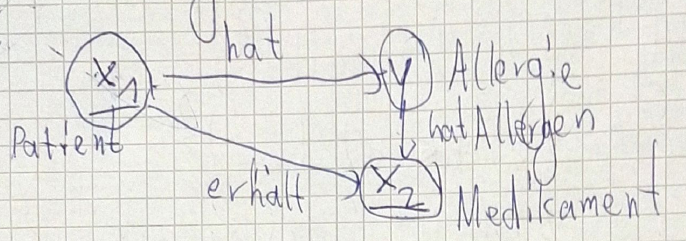
\includegraphics[width=3.81910in,height=1.63200in]{media/75logic.png}

\textbf{T7.6}

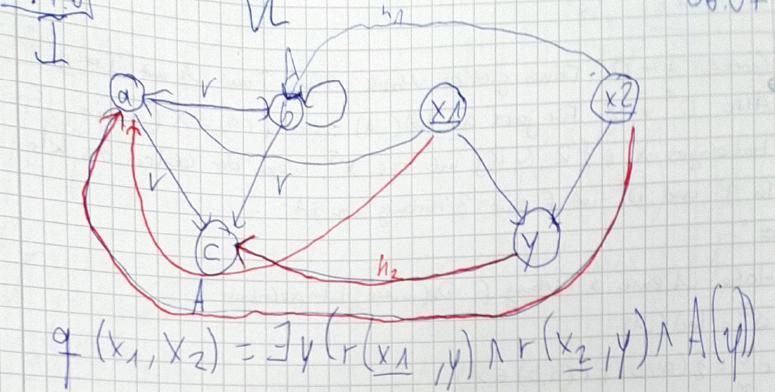
\includegraphics[width=5.81910in,height=3.23200in]{media/76intelog.png}

Homomorph von $q$ auf $\MI$ z.B:

$$x_1 \rightarrow a \quad x_2 \rightarrow b \quad y \rightarrow c$$

$Antwort(a,b)$

oder 

$$x_1 \mapsto a \quad x_2 \mapsto a \quad y \mapsto c$$

Ant(a,a)

und mindestens zwei weitere

\textbf{T7.7}

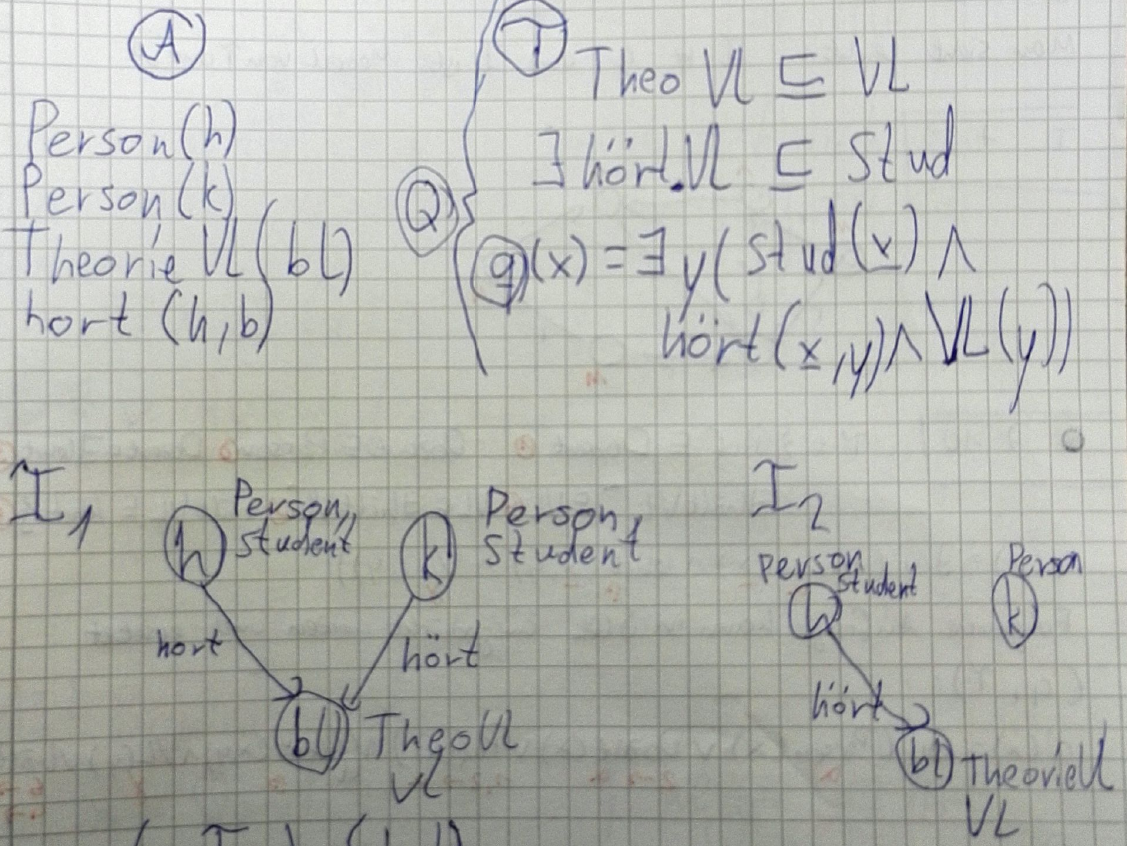
\includegraphics[width=5.81910in,height=5.83200in]{media/77omq.png}

$ans(q, \MI_1) = \{hanna,klaus\}$

$ans(q, \MI_2) = \{hanna\}$

Es gilt: $cert(Q, \MA) = \{h\}$

\textbf{T7.8}

"`$\Leftarrow$"'

Gelte $\MA \not\models Q$. Dann gibt es Modell $\MI$ von $\MT$ und $\MA$ mit $\MI \not\models q$.

Also $D^{\MI} \neq \emptyset$. Für jedes $a \in Ind(\MA)$ setze $f(a) = X$ für ein beliebiges $X \in{R,G,B}$ mit $a \in X^{\MI}$. Wegen der letzten der drei KIs in $\MT$ und $D^{\MI}$ ist $f$ eine 3-Färbung von $\MA$.

"`$\Rightarrow$"'

Habe $\MA$ eine 3-Färbung $f$. Definiere Interpreation $\MI$:

$\Delta^{\MI} = Ind(\MA)$

$r^{\MI} = \{(a,b) | r(a,b) \in \MA \}$

$X^{\MI} = \{a | f(a) = X\}, X \in \{R,G,B\}$

$D^{\MI} = \emptyset$

Man sieht leicht: $\MI \not\models q$ und $\MI$ ist Modell von $\MT$ und $\MA$

\textbf{T7.9}

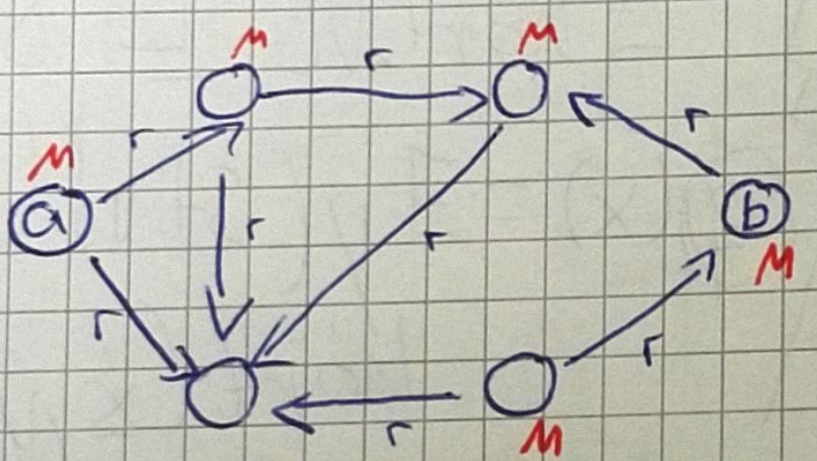
\includegraphics[width=3.81910in,height=1.63200in]{media/79rew.png}

\textbf{T7.10}

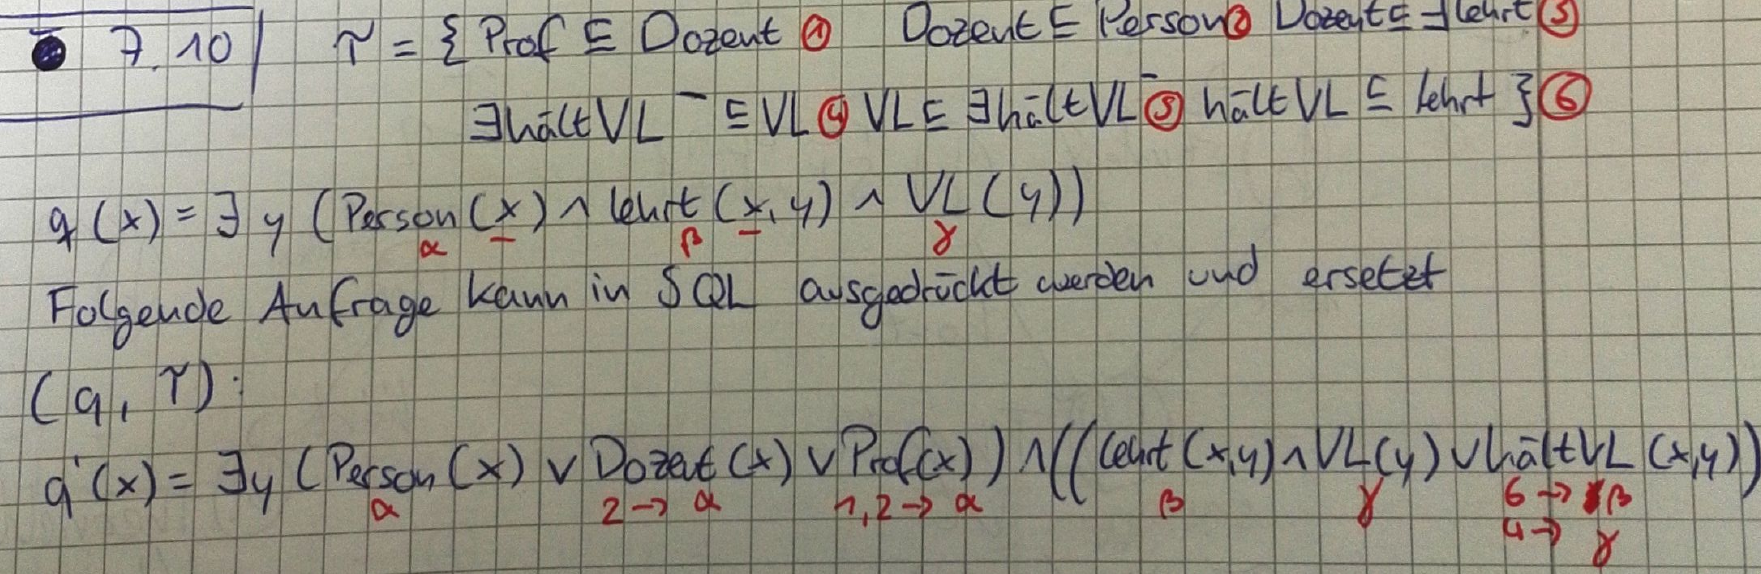
\includegraphics[width=4.81910in,height=2.33200in]{media/710dllite.png}

\textbf{T7.11}

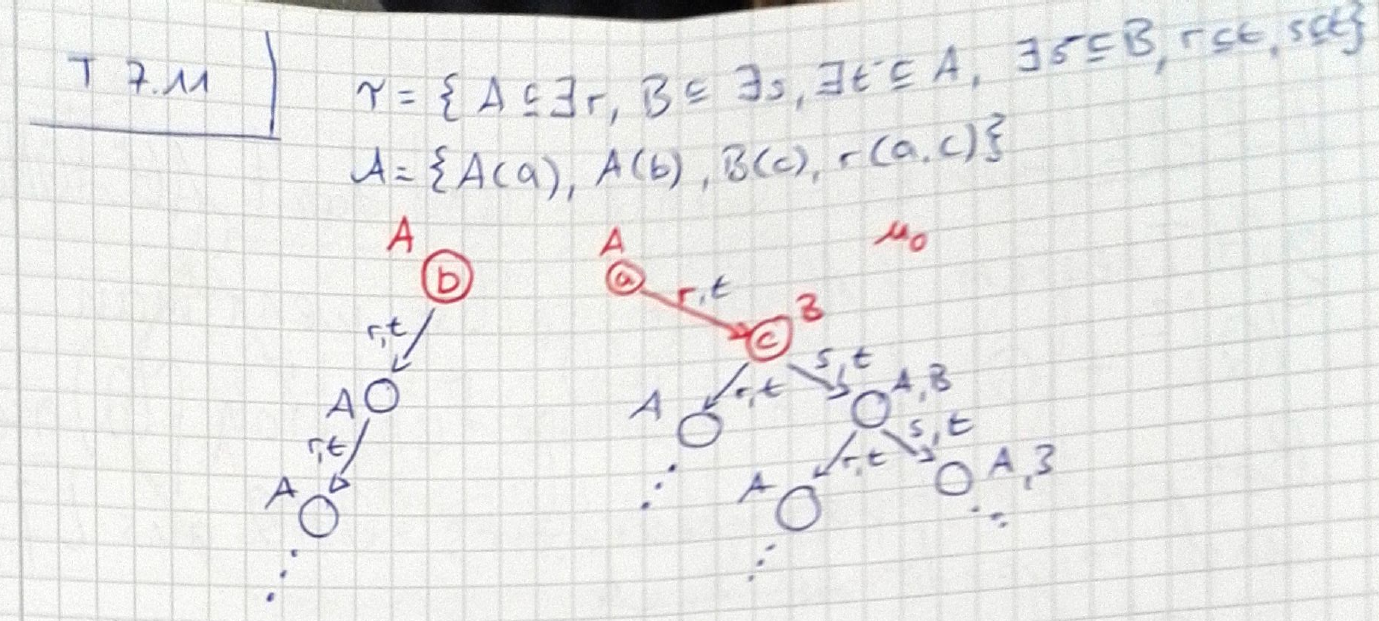
\includegraphics[width=4.81910in,height=2.33200in]{media/711um.png}

\textbf{T7.12}

Für $\EL$-OMQs (und damit $\ALC$-OMQs) gilt Theorem 7.16 nicht, selbst wenn man $|Q|^2 + |Q|$ durch beliebige Funktion $f(Q)$ ersetzt. 

Betrachte Erreichbarkeits-OMQ aus L7.12 und folgende ABox $\MA$

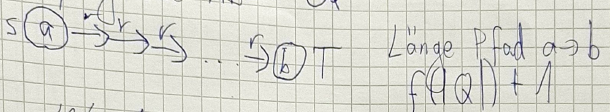
\includegraphics[width=7.41910in,height=1.33200in]{media/712elomq.png}

Es gilt $\MA \models Q$, aber $\MA' \models Q$ für alle $$\MA' \subseteq \MA$$

Nicht Lokalität von Q zeigt sich auch, wenn man naiv versucht, ein Rewriting zu konstruieren:


\includegraphics[width=4.41910in,height=2.33200in]{media/712rew.png}

\textbf{T7.13}

Beweisidee

Wenn $\MA = Q$, dann $\MU \models q$ wegen L7.15.

Per Konstruktionen hat $\MU$ folgende Form:

...
	\newpage

	\section{Übersichten}
	\subsection{Erfüllbarkeit in $\ALC$}

\subsubsection{$\ALC$ bzgl. TBoxen}

Komplexität: ExpTime-vollständig

\paragraph{Obere Schranken}

Um zu zeigen, dass die Erfüllbarkeit von $\ALC$ bzgl. TBoxen in ExpTime liegt, haben wir den Algorithmus ``Typ-Elimination'' eingeführt.

Für diesen habe wir syntaktische Typen definiert und dann gezeigt, dass dieser in $2^\{|C_0|+|\MT|\}$ Schritten terminiert.

Die Korrektheit haben wir gezeigt, indem wir aus den Typen eine Interpretation gebildet haben und gezeigt haben, dass diese ein Modell von $C_0$ bzgl. $\MT$ ist.

Die Vollständigkeit haben wir gezeigt, indem wir semantische Typen aus dem Modell $\MI$ gebildet haben. Dann haben wir (per Induktion über ) gezeigt, dass diese immer eine Teilmenge der Mengen von syntaktischen Typen die bei $\ALC$-Elim gebildet werden.

\paragraph{Untere Schranke}

Nun wollen wir zeigen, das das Erfüllbarkeitsproblem von $\ALC$ ExpTime-hart ist. Dazu reduzieren wir das ExpTime Spiel auf die Erfüllbarkeit von $\ALC$.

\subsubsection{$\ALC$ ohne TBox}

Komplexität: PSpace-vollständig

\paragraph{Obere Schranken}

Um zu zeigen, dass die Erfüllbarkeit von $\ALC$ ohne TBoxen in PSpace liegt, haben wir den Algorithmus ``$\ALC$-Worlds'' eingeführt.

Für diesen haben wir i-Typen definiert und dann gezeigt, dass der Algorithmus terminiert und in PSpace liegt. Dies liegt daran, dass der Algorithmus einen endlichen Baum bildet, und wir nur einen Pfad zur selben Zeit betrachten müssen, da wir per Tiefensuche prüfen.

Korrektheit: Aus dem Rekursionsbaum bilden wir eine Interpreation $\MI$ und zeigen, dass diese ein Modell von $C_0$ ist.

Vollständigkeit: Verwende $\MI$ um die nichtdeterministischen Entscheidungen des Algorithmus zu lenken.

\paragraph{Untere Schranke}

Nun wollen wir zeigen, dass das Erfüllbarkeitsproblem von  $\ALC$ ohne TBoxen PSpace-hart ist. Dies zeigen wir, indem wir das PSpace-Spiel auf die Erfüllbarkeit reduzieren. 

\subsubsection{$\ALCI$, $\ALCQ$, $\ALCQI$}

Für diese Variationen von $\ALC$ gelten die selben Komplexitäten wie für $\ALC$

\subsubsection{Unentscheidbare Erweiterungen}

Wir betrachten hier beispielhaft die Erweiterung von um konkrete Bereiche. Dazu reduzieren wir das Halteproblem für 2-Registermaschinen auf die Erfüllbarkeit dieser Erweiterung.

\subsection{Erfüllbarkeit in $\EL$}

Jedes $\EL$-Konzept ist erfüllbar bzgl. jeder TBox.

\subsection{Subsumtion in $\EL$ ohne TBox}

Subsumtion in $\EL$ kann in polynomieller Zeit entschieden werden:

\begin{itemize}
	\item Konstruiere $\MI_C$ und $\MI_D$ in polynomieller Zeit.
	\item Überprüfe in polynomieller Zeit, ob $(\MI_D,d_W) \precsim (\MI_C,d_W)$
	\begin{itemize}
		\item Berechne maximale Simulation ($|C| \cdot |D|$-Schritte)
		\item Teste ob $(d_w,d_w) \in \rho$
	\end{itemize}
\end{itemize}

\subsection{Subsumtion von Konzeptnamen in $\EL$ bzgl. TBox}

Zunächst wandeln wir eine $\EL$-TBox $\MT$ in linearer Zeit in eine TBox $\MT'$ in Normalform um, die eine konserative Erweiterung von $\MT$ ist. Dazu wenden wir erschöpfend die Regeln NF1 bis NF5 an.

Nun kann der Algorithmus erschöpfend die Regeln R1 bis R4 anwenden. Die Konstruktion von $\MT$ terminiert nach $\mathcal{O}(|\MT|^2)$ vielen Regelanwendungen. Dies wird damit gezeigt, das nur begrenzt viele Konzeptinklusionen gezeigt werden.

Die Korrektheit (Für alle Konzeptnamen $A,B$ gilt: $A \sqsubseteq B \in \MT*$ impliziert $\MT \models A \sqsubseteq B$) wird gezeigt, indem wir zeigen $\MT_i \models \MT_{i+1}$ für alle i = 0, ..., n-1. Dh. soll für alle $C \sqsubseteq D \in \MT_{i+1}$ gelten: $\MT_i \models C \sqsubseteq D$. Dabei argumentieren wir dann durch Analyse der Regeln. 

Für den Beweis der Vollständigkeit (Für alle Konzeptbamen $A,B$ gilt $\MT \models A \sqsubseteq B$ impliziert $A \sqsubseteq B \in \MT *$) definieren wir die kanonische Interpretation $\MI$ wie folgt:

\begin{itemize}
\item
  $\Delta^{I} = \left\{ d_{A}\ |\ A\ \mathrm{\text{Konzeptname\ in\ T}}* \right\} \cup \left\{ d_{\top} \right\}$
\item
  $A^{I} = \left\{ d_{\text{B\ }} \middle| \ B \sqsubseteq A \in T* \right\}$
\item
  $r^{I} = \left\{ \left( d_{A},d_{B} \right)\  \middle| \ A \sqsubseteq A^{'} \in T*\ \mathrm{\text{und}}\ A^{'} \sqsubseteq \exists r.B \in T*,\ A^{'}\ \mathrm{\text{Konzeptname}} \right\}$
\end{itemize}

Zunächst zeigen wir, dass die kanonische Interpretation $\MI$ ein Model von $\MT *$ ist.

Nun können wir die Vollständigkeit zeigen. Dazu zeigen wir die Kontraposition: Für alle Konzeptbamen $A,B$ gilt $A \sqsubseteq B \not\in \MT *$ impliziert $\MT \not\models A \sqsubseteq B$.

\subsubsection{Erweiterungen von $\EL$}

\paragraph{$\EL\mathcal{U}_{\bot}$}

ExpTime vollständig.

Gezeigt per Reduktion auf Konzeptname $A$ bzgl. $ALC$-TBox $\MT$.

Schritt 1: Ersetzte Werterestriktionen in $\MT$ durch Existenzrestriktionen.

Schritt 2: Modifiziere $\MT$ so, dass Negation nur vor Konzeptnamen auftritt:

z.B.: $$A \sqsubseteq \exists s.(B' \sqcup \neg r.B)$$

wird zu

$$A \sqsubseteq \exists s.(B' \sqcup X)$$
$$X \equiv \exists r.B$$

Schritt 3: Entferne Negation vollständig aus $\MT$ 

\begin{itemize}
	\item Ersetze jedes $\neg X$ durch $X'$ mit $X'$ neuer Konzeptname
	\item Erwinge korrektes Verhalten von $X'$:
	$$\top \sqsubseteq X \sqcup X'$$
	$$X \sqcap X' \sqsubseteq \bot$$
\end{itemize}

Zeigen, dass $A$ erfüllbar bzgl. $\MT$ gdw. $A$ erfüllbar bzgl. der entstandenen TBox.

\paragraph{$\EL\mathcal{U}$}

ExpTime-vollständig

Beweis: Reduktion von Erfüllbarkeit von Konzeptname $A$ bzgl. $\EL\mathcal{U}_{\bot}$-TBox $\MT$.

\begin{itemize}
\item Nimm o.B.d.A. an dass $\bot$ nur in der Form $C \sqsubseteq \bot$ vorkommt. Man kann zeigen, das jedes $\EL\mathcal{U}_{\bot}$-Konzept äquivalent zu $\EL\mathcal{U}$-Konzept oder $\bot$ ist. Die Äquivalenzen sind:
$$C \sqcap \bot \equiv \bot$$
$$C \sqcup \bot \equiv C$$
$$\exists r.\bot \equiv \bot$$

Dann sind alle Axiome von der Form:
$$C\sqsubseteq D, \bot \sqsubseteq D, C \sqsubseteq \bot, \bot \sqsubseteq \bot$$

Wobei die Form 2 und 4 immer erfüllt ist und daher gelöscht werden kann.


\item Nun ersetzen wir $\bot$ durch neuen Konzeptnamen $L$

\item und füge $\exists r.L \sqsubseteq L$ für alle Rollennamen $r$ in $\MT$ hinzu.
\end{itemize}

Nun kann man zeigen, das $A$ unerfüllbar bzgl. $\MT$ gdw. $\MT ' \models A \sqsubseteq L$

\paragraph{$\EL^{\forall}$}

ExpTime-vollständig

Reduktion von Subsumition zwischen Konzeptnamen bzgl. $\EL\mathcal{U}$-TBox $\MT$

Wir können annehmen, das Disjunktion nur in den folgenden Formen vorkommt:

\begin{itemize}
	\item $A_1 \sqcup A_2 \sqsubseteq$ wird in $\MT$' durch $A_1 \sqsubseteq A, A_2 \sqsubseteq A$ ersetzt
	\item $A \sqsubseteq B_1 \sqcup B_2$ wird in $\MT$' ersetzt durch $A \sqcap \exists r.\top \sqsubseteq B_1$ und $A \sqcap \forall r.X \sqsubseteq B_2$ mit $r,X$ neu.
\end{itemize}

Nun zeigen wir $\MT \models A \sqsubseteq B$ gdw. $\MT' \models A \sqsubseteq B$

\paragraph{$\EL^{\leq 2}$}

ExpTime-vollständig

Reduktion von Subsumition zwischen Konzeptnamen bzgl. $\EL\mathcal{U}$-TBox $\MT$

Wir können annehmen, das Disjunktion nur in den folgenden Formen vorkommt:

\begin{itemize}
	\item $A_1 \sqcup A_2 \sqsubseteq$ wird in $\MT$' durch $A_1 \sqsubseteq A, A_2 \sqsubseteq A$ ersetzt
	\item $A \sqsubseteq B_1 \sqcup B_2$ wird in $\MT$' ersetzt durch $A \sqsubseteq \exists r.X \sqcap \exists r.Y$, $A \sqcap \exists r.(X \sqcap Y) \sqsubseteq B_1$ und $A \sqcap (\geq 2 r) \sqsubseteq B_2$ mit $r,X$ neu.
\end{itemize}

Nun zeigen wir $\MT \models A \sqsubseteq B$ gdw. $\MT' \models A \sqsubseteq B$

\paragraph{Konvexität}

Jede nicht-konvexe Erweiterung von $\EL$ ist ExpTime-hart

Leider sind aber auch konvexe Erweiterungen nicht zwangsläufig in PTime.

Konvexe Erweiterungen sind Erweiterungen wenn für alle TBoxen $\MT$ und Konzepte $C,D_1,D_2$ gilt:

$\MT \models C \sqsubseteq D_1 \sqcup D_2$ impliziert $\MT \models C \sqsubseteq D_i$ für ein $i \in \{1,2\}$
	\newpage


	\setbibliography

\end{document}
